\documentclass{aicom2e}
\usepackage{amsmath}
\interdisplaylinepenalty=2500
\usepackage[algo2e,ruled,vlined,linesnumbered]{algorithm2e}
\usepackage[active]{srcltx}


\usepackage{amsthm, amssymb,amsfonts}
\usepackage{graphicx}
\usepackage{epsfig}
\usepackage{latexsym}
\usepackage{colortbl}
\usepackage{times}
\usepackage{helvet}
\usepackage{courier}
\usepackage{caption}
\usepackage{subfig}
\usepackage{float}
\usepackage{xcolor}
\usepackage{pslatex}
\usepackage{eso-pic}
\usepackage[bottom]{footmisc}
\usepackage{url}
\usepackage{etex}


\newtheorem{definition}{Definition}
\newtheorem{lemma}{Lemma}
\newtheorem{corollary}{Corollary}

\newtheorem{theorem}{Theorem}
\newtheorem{observation}{Observation}
%\newcommand{\kgs}{$k$-goal problem}
\newcommand{\kgs}{$k$GP}
\newcommand{\kgbfs}{$k$-goal best-first search}


\newcommand{\astar}{A$^*$}
\newcommand{\kastar}{kA$^*$}
\newcommand{\kastarmin}{kA$^*_{min}$}
\newcommand{\kastarmax}{kA$^*_{max}$}
\newcommand{\kxastar}{k$\times$A$^*$}
\newcommand{\astari}[1]{A$^*_#1$}
\newcommand{\newcode}[1]{{\color{blue}[+] #1}}

\newcommand{\minf}{$F_{min}(n)$}
\newcommand{\maxf}{$F_{max}(n)$}
\newcommand{\tuple}[1]{\ensuremath{\left \langle #1 \right \rangle }}
\newcommand{\open}{\textsc{Open}}
\newcommand{\closed}{\textsc{Closed}}
\DeclareMathOperator*{\argmin}{\arg\!\min}
\newcommand{\roni}[1]{\textbf{[RS:#1]}}
%\newenvironment{proof}{\noindent{\bf Proof:~~}}{\qed}

\begin{document}
\begin{frontmatter}                           % The preamble begins here.
%
%\pretitle{Pretitle}
\title{Shortest Path for K Goals}
% \runningtitle{Running title}
%\subtitle{Subtitle}
\maketitle
%
\author[]{Ariel Felner}
\address{Ben Gurion University of the Negev\\ Be'er Sheva, Israel\\
    E-mail: felner@bgu.ac.il}

\author[]{Meir Goldenberg}
\address{The Jerusalem College of Technology\\ Jerusalem, Israel\\
    E-mail: mgoldenbe@gmail.com}
\author[]{Roni Stern}
\address{Ben Gurion University of the Negev\\ Be'er Sheva, Israel\\
    E-mail: roni.stern@gmail.com}

\begin{abstract}
    In this paper we study the $k$ goal search problem (\kgs{}),
    which is the problem of finding the lowest-cost path
    from a given state to $k$ states. Two fundamental approaches
    are presented: searching for the $k$ goals one at a time,
    or searching for all $k$ goals together in a single pass of the
    search space. We call the latter approach \kastar{}
    and describe several ways it can be implemented.
    We lay the theoretical foundation for analyzing \kgs{} problems
    and perform an empirical evaluation to demonstrate
    its applicability.
\end{abstract}

\begin{keyword}
artificial intelligence\sep AI\sep Heuristic Search
\end{keyword}
%
\end{frontmatter}

\section{Introduction}

% SPP is classical, important and super general

The shortest path problem (SPP) in a graph is a fundamental problem in Computer
Science, with many applications in Artificial Intelligence and Operations
Research. The input to an SPP problem is a graph and two vertices -- a {\em
start} vertex and a {\em goal} vertex -- and the task is to find the
lowest-cost path in the graph from start to goal. Classical algorithms such as
Dijkstra's algorithm~\cite{DIJ59} and \astar{}~\cite{hartNR68Astar} have been
proposed for solving SPP. SPP algorithms have been applied to various types of
graphs. In some cases, the graph is given explicitly, e.g., representing
roadmaps, grids and game maps~\cite{sturtevant2012benchmarks}. In other cases,
the graph is defined implicitly by an initial vertex and a set of transition
functions, e.g., representing a space of possible robot configurations, puzzle
permutations, or STRIPS-like states in a domain-independent planning problem.
%[[AF: do we want references?]]\roni{Sure, any ideas what to add here?}


% We talk about k SPP

This paper addresses a generalization of SPP, where the task is to solve $k$
SPP problems, such that all the problems share the same start vertex. That is,
we have a single start state and $k$ goal states, and the task is to find $k$
shortest paths, where each path is a shortest path from the start state to a
different goal state. We denote this problem as the {\em $k$-goal} problem
(\kgs{}).


% k-goal is not TSP

\kgs{} is similar but different from previously studied tasks such as the
traveling saleman problem (TSP) and incremental
search~\cite{koenig2004lifelong}. In TSP, the task is to find a single path
that passes through a set of vertices. By contrast, in \kgs{} we aim for $k$
paths, one per goal. In incremental search we have a single goal but the
underlying graph changes. By contrast, in \kgs{} the underlying graph is static,
but we are given $k$ goals upfront. % and the task is to find paths for all these goals.


% Motivation 1. Star-shaped tour

\kgs{} has many applications. Assume a tour planning application. It is common
to prefer staying in the same hotel when visiting a city, visiting different
sites in different days but returning every night to the same hotel to avoid
packing and unpacking. Path planning under this constraint is thus a \kgs{}
instance, as we have a single common start state and multiple goal states.

% Motivation 2. Choosing between multiple sites

A related example for \kgs{} occurs when planning a family vacation. Assume
that there are $k$ amusement parks and the family wishes to stop in one of
them. It is hard, or even impossible, to exactly model the preferences of the
different family members, but clearly the cost of getting to each of the
different amusement parks is an important consideration for the family members
to know about. Here too, we have a \kgs{} problem, where the start state is the
family's home and the goals are the different amusement park. This represents a
more general scenario that occurs when developing an intelligent personal
assistant, where the planning component may be decoupled from the agent's
high-level decision making component, e.g. when following a
Believe-Desire-Intention (BDI)
architecture~\cite{bratman1999intention,georgeff1998belief}. In such cases
there may be multiple goals an agent may wish to achieve and the cost of
reaching them is important input to the agent's decision making module.


Efficient solutions to the $k$-goal problem can be helpful in many robotic
challenges. For example, consider the task of deploying multiple drones from a
a central dispatcher location to $k$ locations. Another robotic application
where the search for $k$ goals is needed is when using the Incremental Roadmap
Spanner technique~\cite{marble2013asymptotically}, which is a motion planning
technique that includes searching for the shortest path to a limited number of
nearby locations. In fact, preliminary work on using heuristic search to solve
\kgs{} was done exactly for this problem~\cite{DobsonB14}.
%[[AF: state exactly which of our versions they used. For example, say: they used a variant of the KMIN algorithm presented below.]]\roni{We can't say that here because we did not introduce our algorithms.  But it is good to say that later TODO}

A trivial solution to \kgs\ is to independently run a SSP solver $k$ times. We
analyze the runtime of this option and identify potential redundancies. Then,
we propose an alternative approach where a single search algorithm is used to
search for all the $k$ goals together, avoiding some of these redundancies. We refer
to this framework as \kastar{}. Implementing \kastar{} includes several design
choices, such as how to aggregate multiple heuristic estimates and what to do
after an optimal path to one of the goals is found. We analyze the theoretical
properties of these different design choices and point out their pros and cons.
Then, we provide a theoretical and experimental study that compare the
\kastar{} approach and the simpler, independent $k$ searches approach,
providing useful guidelines for when to use which option.

%\roni{We need to think about the term {\em concurrent} in our context. I fear it will seem that we are talking about parallel computation.}
%\roni{TODO: SOME RELATED WORK? AF: which one?}

\section{Background and Problem Definition}

%In this section, we formally define the $k$-goal search problem.

% Graphs, costs, SSP
To improve readability, we provide Table~\ref{tab:notations}, which
summarizes some of the key notations introduced throughout the paper .
Let $G=(V,E,w)$ be a weighted graph, where $V$ is the set of vertices, $E$ is
the set of edges, and $w:E\rightarrow \mathbb{R}^+$ is a function that assigns
a non-negative real value to each edge. This value is referred to as the {\em
cost} of the edge. The cost of a path in a graph is the sum the edge costs
along it. In the Artificial Intelligence literature, graphs are often used to
represent state spaces, where the graph vertices represent possible states of
the world, the out-going edges of a vertex represent possible actions that an
agent can perform at the corresponding state, and the cost of an edge
represents the cost of the corresponding action. Thus, throughout this paper we
will use the terms {\em states} and {\em actions} instead of vertices and
edges, respectively, and use the term {\em applying an action} instead of
traversing an edge. Note that a path in a graph corresponds to an applicable
sequence of actions.

\begin{definition}[The Shortest Path Problem (SPP)]
A shortest path problem (SPP) is defined by a tuple $\tuple{G,s,g}$, where $s$
and $g$ are states in $G$ and the problem is to find the lowest cost path in
$G$ from $s$ to $g$. \label{def:spp}
\end{definition}

\subsection{The \astar{} Algorithm}




\begin{algorithm2e}[t!]
    \small
    \KwIn{Start state $s$, Goal state $g$)}
    $g(s)\gets 0$; \open{}~$\gets\emptyset$; \closed{}~$\gets \emptyset$\\
    Add $s$ to \open{} with key $f(s)=g(s)+h(s)$\\
    \While {\open{} $\neq \emptyset$} {
        $best \gets $ a state from \open{} with the smallest key \nllabel{line:open:chooseNode}\\
        Move $best$ from \open{} to \closed{}\\
        \If {$best$ is the goal}{\Return the lowest-cost path found to $best$}
        \For{every action $A$ applicable at state $best$ \nllabel{line:nextNeighbor}}{
            $c \gets $ generate a state by applying $A$ to $best$ \nllabel{line:astar:generate-start}\\
            $g_{new}\gets g(best)+w((best,c))$\\
            % Duplicate detection
            \If{$c$ in $\open{}\cup \closed{}$ \nllabel{line:dd-start}}{
                \If{$g(c) \leq g_{new}$}{
                    {\bf continue} (goto line~\ref{line:nextNeighbor})
                }
                Remove $c$ from \open{} and \closed{}  \nllabel{line:dd-end}\\
            }
            % Update n's g and f values
            $g(c)\gets g_{new}$ \nllabel{line:compute-f}\\
            Add $c$ to \open{} with key $f(c)=g(c)+h(c)$  \nllabel{line:astar:generate-end}\\
        }
    }
    \Return No solution exists\\
    \caption{\astar{}}
    \label{alg:astar}
\end{algorithm2e}



% A* for single agent search
SPP has been well-studied in the literature. \astar{}~\cite{hartNR68Astar} is a popular
 heuristic search algorithm for solving SPP. For completeness, we provide a short description of \astar{}
 and provide its pseudo code in Algorithm~\ref{alg:astar}. \astar{} maintains two lists of states: \open{} and
\closed{}. Initially, \closed{} is empty and \open{} contains only the start
state ($s$). Every state that is added to \open{} is associated with a $g$
value and an $f$ value. The $g$ value of a state $n$, denoted $g(n)$, is the
cost of the lowest cost path found so far from the start state $s$ to $n$.
Hence, $g(s)$ is set to zero.
The $f$ value of $n$, denoted $f(n)$, is the sum
of $g(n)$ and a heuristic estimate of the cost of the lowest cost
path from $n$ to the goal state $g$. This heuristic estimate is denoted
by $h(n)$. %, and there is an abundance of prior work in the literature on how to develop heuristics that

%[[AF: In all our previous paper we always used $g$-value and $f$-value etc. Please change to this notation unless you really do not want to]]\roni{I really do not want to}

In every iteration of the main loop of \astar{}, the state with the lowest $f$ value in \open{}
is moved from \open{} to \closed{}. If that state is a goal, the search halts
returning the path found to it.\footnote{We omit in this pseudo code how
back-pointers are maintained to  preserve the best path to each state.}
Otherwise, the state is {\em expanded}. Expanding a state $n$ means generating
every state that can be reached by applying a single action at state $n$. Then,
the $g$ and $f$ values of every generated state $c$ are computed based on the
$g$ value of its parent, the cost of the action used to generate $c$, and the
heuristic estimate $h(c)$. Finally, the generated states are added to \open{}
with their $f$ values, to be considered for expansion in future iterations. If
the searched graph is not a tree, multiple paths to the same state may be
explored. To address this, \astar{} keeps track of the states it has generated
and maintains for every state only the best (lowest cost) path found to it (lines~\ref{line:dd-start}-\ref{line:dd-end}).


%\roni{TODO: Maybe add more line numbers to the text?} \roni{TODO: Add something on tie breaking [[AF: do not do any of these]]}






% A* properties and admissible heursitics

\astar{} has several important properties. First, if the heuristic used is {\em
admissible}, i.e., it does not over-estimate the cost of the lowest cost path
to the goal, then \astar{} is guaranteed to solve SPP, i.e., to return a lowest
cost path from $s$ to $g$.\footnote{In fact, it is sufficient that the
heuristic is admissible only for the states that are on a single lowest-cost
path for \astar{} to guarantee
optimality~\cite{karpas2012optimal,dechter1985generalizedBestFirst}.} Second,
if the heuristic is {\em consistent} then \astar{} is guaranteed to never
expand a state more than once~\cite{hartNR68Astar}.
%when a state $n$ is expanded it is guaranteed that the lowest cost path from $s$ to $n$ has been found, and thus $g(n)$ is the cost lowest cost path from $s$ to $n$.
\begin{definition}[Consistent Heuristic~\cite{hartNR68Astar}]
    A heuristic $h$ is {\bf consistent} if for every pair of states $x$ and $y$
    it holds that $h(x)\leq d(x,y)+h(y)$, where $d(x, y)$ is
    the cost of the lowest-cost path from $x$ to $y$.
    \label{def:consistent}
\end{definition}



%The important implication of a consistent heuristic is that \astar{} with a consistent heuristic is guaranteed to expand every state at most once.

Third, under some conditions, it can be shown that up to tie-breaking between
states with equal $f$ values, \astar{} will only expand the minimal set of
states required to find an optimal
solution~\cite{dechter1985generalizedBestFirst}. A recent variant of \astar{}
provides a similar guarantee with respect to the number of states generated as
well~\cite{goldenberg2013optimal}. This type of guarantees, often referred to
as the {\em optimally effective} property of \astar{}, is  important because in
many cases the runtime of the algorithm is correlated with the number of states
expanded/generated. Thus, guaranteeing that \astar{} expands/generates the
minimal number of states provides some sort of optimality guarantee for
\astar{}'s efficiency compared to other equally informed algorithms.

%[[AF: not sure what is the point in the last sentence. In fact, the A* section can be significantly squeezed.]]\roni{1. I don't see a reason to squeeze the \astar{} section. This paper addresses a simple enough topic that it should be easily accessible to non-search people as well. 2. The last sentence aims to say that \astar{} is optimally effective and why this is important but without committing to the exact details of optimality}

\subsection{The $k$-Goal Problem}

In this paper we focus on the \kgs{} problem, which can be viewed as a generalization of SPP.

%\begin{definition}[$k$-goal search]
%   A \kgs\ problem is defined by a tuple $\tuple{G,s, g_1, g_2, \ldots, g_k}$,
%   where $s$ and $g_1, g_2, \ldots, g_k$ are states in $G$ and the problem is to find
%   $k$ paths $p_1,\ldots p_k$ such that for every $i\in [1,k]$ it holds that $p_i$ is a lowest-cost path from $s$ to $g_i$.
%   \label{def:k-goal}
%\end{definition}


\begin{definition}[$k$-goal problem]
A \kgs\ problem is defined by a tuple $\tuple{G,s, \textbf{g}}$ where $G$ is a
graph $s$ is state in $G$, and $\textbf{g}=(g_1,g_2,\ldots,g_k)$ is a vector of
$k$ states. A solution to the \kgs{} problem is a vector of $k$ paths
$\textbf{p}=(p_1,\ldots p_k)$ such that for every  $i\in [1,k]$ it holds that
$p_i$ is a lowest-cost path from $s$ to $g_i$. \label{def:k-goal}
\end{definition}


% k searches independentaly

%[[AF: I do not like your notation for vectors. I prefer overline. Your call]] \roni{I saw both in many papers. But mostly I saw the bold notation (although I am used to the overline from school). Keeping it as is.}

Clearly, SPP is a special case of \kgs\ with $k=1$. A trivial solution to \kgs\
is to consider it as $k$ independent SPPs and use \astar{} (or any other SPP
algorithm) multiple times to solve these $k$ problems. In the next section we
present this approach and analyze its complexity. In later sections we
introduce a different approach that activates a single search that aims to find the lowest-cost path
to all $k$ goals in a single pass of the state space. This allows re-using information
between the $k$ different tasks, potentially decreasing the overall search
effort.


\section{$k$ Independent Searches}
\label{sec:k-one-goal}
\begin{algorithm2e}[t!]
    \small
    \KwIn{Start state $s$, Goals vector $\textbf{g}=(g_1,\ldots g_k$)}
    \textsc{Solution}$\gets \emptyset$\\
    \For{$i$=1 to $k$}{
        $p_i\gets$ \astar{}($s$,$g_i$)\\
        Add $p_i$ to \textsc{Solution}\\
    }
    \Return \textsc{Solution}\\
    \caption{\kxastar{}: \kgs{} with $k$ \astar{}s}
    \label{alg:k-searches}
\end{algorithm2e}




Algorithm~\ref{alg:k-searches} outlines the trivial approach for solving
\kgs{}: running \astar{} $k$ times, one for each of the $k$ goals. The
resulting $k$ paths are returned as a solution to the \kgs{} problem. We refer
to Algorithm~\ref{alg:k-searches} as \kxastar{}.


To analyze the effectiveness of \kxastar{}, we use the notions of {\em surely necessary} states and {\em surplus} states~\cite{dechter1985generalizedBestFirst,goldenberg2014enhanced}.
%\roni{Meir and Ariel: who used this term before us?}

\begin{definition}[Surplus States and Surely Necessary States]
    Let $\Pi$ be a SPP defined by the tuple $\tuple{G,s,g}$, and let $opt_\Pi$ denote the cost of an optimal solution to $\Pi$.
    A state $n$ is called a {\em surly necessary} state with respect to $\Pi$ if $f(n)<opt_\Pi$
    and it is reachable from $s$ via a path that consists of states with $f$ value lower than $opt_\Pi$.
    A state $n$ is called a {\em surplus} state with respect to $\Pi$ if $f(n)>opt_\Pi$.
\label{def:surplus}
\end{definition}
Without any additional knowledge of the graph $G$, one needs to expand every surely necessary state in order to solve a given SPP,
and one can solve a given SPP without expanding any surplus state~\cite{dechter1985generalizedBestFirst,goldenberg2014enhanced}.
\astar{} does exactly that: expands all necessary states but never expands any surplus state~\cite{dechter1985generalizedBestFirst}.


Consequently, if $\Pi_i$ is the SPP problem from $s$ to $g_i$
then using \kxastar{} to solve \kgs{} will end up expanding every state that is necessary w.r.t at least one of the $k$ SPP problems $\Pi_1,\ldots \Pi_k$ and never expand any state that is surplus w.r.t all these SPP problems.
Hence, one might think that \kxastar{} is ``optimally effective'' for \kgs{},
expanding exactly the set of states one must expand in order to solve the problem, up to tie-breaking between states with the same $f$ value.


This conclusion is not accurate, however, as it overlooks two potential sources for improvement:
\begin{itemize}

\item {\bf Learning from experience.}

When solving one of the $k$ SPP problems (e.g., for finding the optimal path for $g_1$),
one gains additional knowledge of the searched graph, which may be used when solving the subsequent
SPPs for the other goals. For example, propagating heuristic values of states between searches to different goals.
%Such knowledge might be propagation of heuristics of states between searches to different goals.

\item {\bf Avoiding expanding a state multiple times.}

The same state can be generated and expanded in multiple SPPs. For example, \kxastar{}
generates the children of the start state at least $k$ times.
This introduces redundancy to the search process that may be avoided.
\end{itemize}

The first source of improvement is related to the literature on incremental
search~\cite{koenig2004lifelong} and to moving-target search
algorithms~\cite{ishida1995moving,koenig2007speeding}. See
Section~\ref{sec:related-work} for details. In this work we focus on the latter
source of improvement. That is, we aim to avoid expanding a state multiple
times when it is needed for finding the lowest cost path to more than one goal.

%in the search process.
%Next, we analyze these redundancies in the search process that are due to such duplicates.

\subsection{An Analysis of Redundancies in \kxastar{}}
The main source of inefficiency in \kxastar{} is that the sets of states
generated by the individual \astar{} may intersect. This indicates
that some states will be generated in more than one of the $k$ searches.
Since generating a state incurs a computational cost (see Section~\ref{sec:theoretical-analysis} for more details on this),
generating the same state multiple times should be avoided.

\begin{figure}
    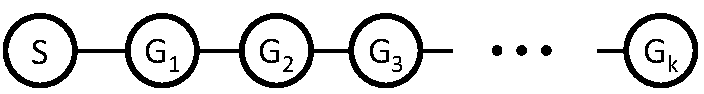
\includegraphics[width=\columnwidth]{k-search-bad_cropped}
    \caption{An example where the $k$ search approach is inefficient.}
    \label{fig:k-search-bad}
\end{figure}
%[[AF: have the goals in the figure be small g not capital]]
An extreme example of this inefficiency is depicted in
Figure~\ref{fig:k-search-bad}. The searched graph is a simple line, where $g_1$ is adjacent to $s$,
$g_2$ is adjacent to $g_1$, and so on. In this case \kxastar{} would generate
$1+2+3+\cdots+(k+1)=\frac{k(k+1)}{2}$ states while it is easy to see that
generating $k$ states would be sufficient to solve the \kgs{} for this case.
In the next section we propose an algorithm that attempts to reduce such redundancies. %for solving the \kgs{}  and method for doing so.




\begin{table}
    \scriptsize
\begin{tabular}{|m{1cm}|m{5.5cm}|}
        \hline
        $\Pi_i$     & The SSP problem of finding a path to goal $g_i$. \\
        $opt_\Pi$   & Denotes the cost of an optimal solution to $\Pi$.\\
        \astari{i}  & An \astar{} for finding the lowest cost path to goal $g_i$. \\
        $f(n)$      & The evaluation function used by \astar{}: $f(n)=g(n)+h(n)$ \\
        $F(n)$      & The evaluation function used by \kastar{} \\

        %A state evaluation function used by \kastar{} to prioritize \open{}. $F(n)$ aggregates a vector of $k$ possibly different $f$ values to a single value. \\
%       \minf{}, \maxf{} & \minf{}=$\min_{j\in[1,k] f(n)}$ and \maxf{}= $\max_{j\in[1,k] f(n)}$\\
        \kastarmin{} & \kastar{} that uses \minf{} to compute its $F$ values\\
        \kastarmax{} & \kastar{} that uses \maxf{} to compute its $F$ values\\
        $h^*_i(n)$ & The cost of the lowest cost path from $n$ to $g_i$\\
        Gen($X$)    & The states generated by algorithm $X$ \\
        $Gen_i(\text{\kastar{}})$ & The states generated by \kastar{} until $g_i$ is expanded \\
        $\open{}_i(X)$ & The number of states in \open{} when algorithm $X$ expanded goal $g_i$\\
        Exp($X$)    & The states expanded by algorithm $X$ \\
        Time($X$)   & The runtime required to run algorithm $X$ \\

        \hline
    \end{tabular}
\caption{This table summarizes some of the notations used in this paper.}
\label{tab:notations}
\end{table}


\section{A Single Search for all  $k$ Goals}
\label{sec:one-k-goal-search}

In this section we generalize \astar{} to search for $k$ goals in a single pass of the search space (the states generated during the search). We
call the resulting algorithm \kastar{}. Before presenting a complete pseudo
code for \kastar{}, we highlight several aspects that differentiates it from \astar{}.

\subsubsection*{Multiple heuristics per state.}


When a state $n$ is generated, \kastar{} computes a $k$-ary vector
$\textbf{h}(n)=(h_1(n),\ldots h_k(n))$, where $h_i(n)$ is the heuristic
estimate of the cost to get from $n$ to goal $g_i$.
We assume throughout this paper that $h_1,\ldots,h_k$ are all admissible heuristics.
These $k$ heuristic values
are used to form a $k$-ary vector $\textbf{f}(n)=(f_1(n),\ldots f_k(n))$, where
$f_i(n)=g(n)+h_i(n)$. We discuss later how the elements of this $k$-ary vector
of $f$ values are aggregated to a single value denoted $F(n)$ -- which is used
to prioritize
% by taking their minimum or their maximum.
\open. That is, in every iteration \kastar{} selects from \open{} a state with
the lowest $F$ value. Note that the computational effort of generating a state
in \kastar{} is larger than that of regular \astar{}, as it requires computing
$k$ heuristics.

%computing $F$ costs more than computing an individual $f$ value, as it at least $k\cdot C_h$, and thus the computation cost of generating a state in \kastar{} is larger than that of \astar{} by $(k-1)\cdot C_{h}$.\footnote{As discussed later in the paper, the actual computational cost in \kastar{} can be smaller, since as the search progresses the list of relevant goals becomes smaller, and consequently computing $F$ becomes easier.}

\subsubsection*{Maintaining the set of active goals}

In \astar{} when a goal is expanded the search halts. By contrast, in \kastar{}
the search does not halt until a lowest-cost path to each of the $k$ goals is
found. To this end, \kastar{} tracks the set of goals for which the lowest-cost
path to them has not been found. This set of goals is referred to as the set of {\em
active goals}. Maintaining the set of active goals is also used to avoid
redundant heuristic computations: when a state is generated we compute the
heuristics only for goals that are still active, which may result in further enhancements (see Section~\ref{sec:lazy}).



%\subsubsection*{Node evaluation function.} When searching for a single lowest-cost path with \astar{}, the state are popped from \open{} according to their $f=g+h$ values. In \kastar{}, we compute the $h$-value forand associate every state in \open{} with a value that considers the $h$-value for each of the $k$ goals.     Thus, when a state is generated then we compute the heuristic for each of the $k$ goals.





\begin{algorithm2e}[t!]
    \small
    \KwIn{Start state $s$, goal states $g_1,\ldots,g_k$}
    $g(s)\gets 0$; \open{}~$\gets\emptyset$; \closed{}~$\gets \emptyset$; \textsc{Solution}$\gets \emptyset$\\
%    {\color{blue}[+] {\tt ActiveGoals} $\gets \{g_1,\ldots,g_k\}$ \nllabel{line:init-active-goals}} \\
    \newcode{{\tt ActiveGoals} $\gets \{g_1,\ldots,g_k\}$ \nllabel{line:init-active-goals}}\\
    \newcode{ $F\gets$ ComputeF(s, ActiveGoals) \nllabel{line:compute-f-start}}\\
    Add $s$ to \open{} with key {\color{blue} $F(s)$}\\
    \While {\open{} $\neq \emptyset$ and {\color{blue}{\tt ActiveGoals} $\neq \emptyset$}} {
        $best \gets$ a state in $\open{}$ with the smallest key \nllabel{kastar:line:open:chooseNode}\\
        Move $best$ from \open{} to \closed{}\\
        \newcode{
        \If {$best\in$ {\tt ActiveGoalsls}}{
            \newcode{Add the path to $best$ to \textsc{Solution} \nllabel{line:storePath}}\\
            \newcode{Remove $best$ from {\tt ActiveGoals} \nllabel{line:removeGoal}}
        }}
        \For{every action $A$ applicable at state $best$  \nllabel{kastar:line:nextNeighbor}}{
            $c \gets $ generate a state by applying $A$ to $best$ \\
            $g_{new}\gets g(best)+w((best,c))$\\
            % Duplicate detection
            \If{$c$ in $\open{}\cup \closed{}$ }{
                \If{$g(c) \leq g_{new}$}{
                    {\bf continue} (goto line~\ref{kastar:line:nextNeighbor})\\
                }
                Remove $c$ from \open{} and \closed{} \\
            }
            % Update n's g and f values
            $g(c)\gets g_{new}$ \nllabel{line:compute-f}\\
            \newcode{$F\gets$ ComputeF(n, {\tt ActiveGoals}) \nllabel{line:computeF}} \\
            \newcode{Add $c$ to \open{} with key $F(c)$}  \\

        }
    }
    \newcode{ \If{{\tt ActiveGoals} $= \emptyset$}{
        \newcode{\Return \textsc{Solution}}\\
    }}
    \Return No solution exists\\
    \caption{\kastar{}}
    \label{alg:kastar}
\end{algorithm2e}



Algorithm~\ref{alg:kastar} shows the pseudo code for \kastar{}.
We highlighted the differences between the pseudo code of \astar{} (Algorithm~\ref{alg:astar})
and the pseudo code of \kastar{} (Algorithm~\ref{alg:kastar})
by marking every line that was changed or modified with a prefix ``[+]'' and the color blue.
Initially, all goals are inserted into the set of active goals, denoted  {\tt ActiveGoals}
(line~\ref{line:init-active-goals} in Alg.~\ref{alg:kastar}). Every state
$n$ that is added to \open{} is associated with a value $F$ that is
computed by the {\tt ComputeF} function (lines~\ref{line:compute-f-start} and~\ref{line:computeF}).\footnote{Note that {\tt ComputeF} accepts the set of active goals. This is done so as to consider only the heuristics to these states when computing the $F$ value.} In every iteration, the state with
the smallest $F$ value is selected and removed from \open{}
(line~\ref{line:open:chooseNode}). If it is a goal then we store the path to it
(line~\ref{line:storePath}). In addition, we remove that goal from the {\tt
ActiveGoals} list, to mark that we are no longer looking for a path to that
goal (line~\ref{line:removeGoal}). When the {\tt ActiveGoals} list is empty, we
halt the search, having found a path to each goal.


\kastar{} (Algorithm~\ref{alg:kastar}) only move a state to \closed{} after
generating its children, and it only halts if \open{} is empty or all paths have been found. Therefore, it is sound and complete, in the sense that if there are paths to the $k$ goals then they will be found, and the paths returned by the algorithm are all valid paths to the $k$ goals. A key question is whether each of these $k$ paths is indeed
an optimal path to its corresponding goal.
As we show next, this depends on how $F$ is computed, as encapsulated in the {\tt
ComputeF} function (lines~\ref{line:compute-f-start} and~\ref{line:computeF}).

%[[AF: In line 23, don't you want to return some of the paths if you have them?]]\roni{I think this will just confuse. The problem is defined for all the $k$ paths.}

\subsection{An Evaluation Function for \kastar{}}

%In \astar{} for a single goal, states are prioritized in \open{} according to the $f=g+h$ value of a state. In contrast, a state in \kastar{} has a vector of $k$ heuristic values $\textbf{h}(n)$ and consequently a vector of $f$ values $\textbf{f}$(n) that contains one $f$ value per goal. Therefore, \kastar{} requires a state evaluation function that aggregates these $f$ values in some way. In Algorithm~\ref{alg:k-goal-bfs} this is encapsulated in the {\tt ComputeF} function. We refer to the value ($F$) returned by this function as the state's $F$ value, and consider the following two options for computing it.
We consider the following two options for computing the $F$ value of a state:
\begin{align}
\text{\minf{}}=&\min_{i\in [1,k]}f_i(n) \\
\text{\maxf{}}=&\max_{i\in [1,k]}f_i(n)
\end{align}
\kastar{} that uses \minf{} as the state evaluation function ($F(n)$) is referred to hereinafter as \kastarmin{}, and similarly \kastar{}
that uses \maxf{} is referred to as \kastarmax{}.



Like many other best-first searches, \kastar{} only removes a state from \open{} after generating its children. Therefore, the following invariant holds regardless of how the $F$ values are computed.
\begin{lemma}
    In every iteration of \kastar{}, it holds that
    for every goal $g_i$ for which the optimal path to has not been found,
    there must exist a state $n$ in \open{} such that $n$ is on an optimal path
    to $g_i$ and $g(n)=g^*(n)$, where $g^*(n)$ denote the cost of the lowest cost path from $s$ to $n$.
    \label{lem:simple}
\end{lemma}
Lemma~\ref{lem:simple} can be proven by induction over the iterations of \kastar{},
since it trivially holds in the first iteration and whenever a state is expanded it generate its children.


\begin{theorem}[\kastarmin{} is admissible]
When \kastarmin{} expands a goal state then the optimal path to that goal has been found.
    \label{the:min-f}
\end{theorem}
 \begin{proof}
    By negation, assume that $g_i$ was expanded, but there is
    a better path to $g_i$ that has not yet been discovered. Due to Lemma~\ref{lem:simple}, we have that as long as the optimal path to $g_i$ has not been found then
    \open{} must contain at least one state $n$
    that is on a better path to $g_i$ and has not been expanded yet. Since $h_i$ is admissible, we have that:
    \begin{equation}
    g(n)+h_i(n)<g(g_i)
    \label{eq:proof-1}
    \end{equation}
    Since $g_i$ was chosen to be expanded before $n$, it must have a $F_{min}$ value no-larger than $n$, i.e.,
    \begin{align}
    F_{min}(n) &\geq  F_{min}(g_i) \\
    g(n)+\min_{j\in [1,k]}h_j(n)& \geq  g(g_i)+\min_{j'\in [1,k]}h_{j'}(g_i)
    \end{align}
    Since $h_i(g_i)=0=\min_{j\in [1,k]}h_j(n)$ then
    \[ g(n)+\min_{j\in [1,k]}h_j(n) \geq  g(g_i) \]
    Finally, since $h_i(n)\geq \min_{j\in [1,k]} h_j(n)$, it holds that
    \[ g(n)+h_i(n) \geq  g(g_i) \]
    contradicting Equation~\ref{eq:proof-1}.
\end{proof}

A direct corollary of Theorem~\ref{the:min-f} is that \kastarmin{} will return the optimal solution to all $k$ paths as required, since it halts after all goal states were expanded.



%\subsection{$F_{max}$}

\begin{figure}
 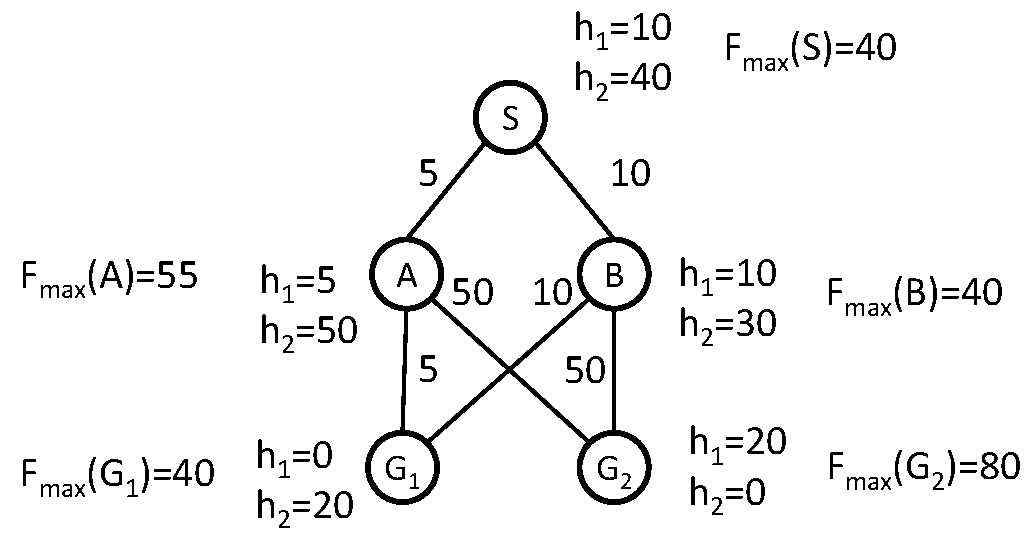
\includegraphics[width=0.9\columnwidth]{max-bad_cropped.pdf}
 \caption{An example of where using \kastarmax{} returns a non-optimal solution. Using \kastarmax{} results in the following expansion order: $S$, $B$, $g_1$.
 Thus, when $g_1$ is expanded, the best path known to it costs 25, while a
 better path to $g_1$ goes through $A$ and costs only 10.}
 \label{fig:max-bad}
 \end{figure}

 \begin{observation}[\kastarmax{} is not admissible]
    Running \kastarmax{} may return a path $\pi_i$ from $s$ to $g_i$ that is not optimal.
    \label{obs:max-f-inadmissible}
 \end{observation}

%[[AF: in the theory above you talked about Fmin and here you talk about kastamx. Use kastarmin too.]]\roni{Maybe you looked at an old version?}

To demonstrate Observation~\ref{obs:max-f-inadmissible}, consider the graph in
Figure~\ref{fig:max-bad}. In this example, using \kastarmax{} results in the
following expansion order: $S$, $B$, $g_1$, and $g_2$. Importantly, state $A$ was not expanded, and so the best path returned for $g_1$ goes
through $B$ and costs 20. A better path to $g_1$ exists, which passes through $A$ and costs only 10.


 % MAX-F is OK for consistent heuristics


The observant reader may have noticed that the heuristic function in
Figure~\ref{fig:max-bad} is inconsistent (Definition~\ref{def:consistent}):
$h_2(A)=50$ while its child, $g_1$, is connected to it via an edge of
cost 5 and has $h_2(g_1)=0$. If $h$ was consistent then $h_2(A)\leq
h_2(g_1)+w((A,g_1))$ (recall that $w((A,g_1))$ is the cost of the edge between $A$ and $g_1$).
Interestingly, if the heuristic used is consistent then \kastarmax{} is admissible, as proven in the following result. %below. % using \maxf{} is possible [[AF: admissible?]], [[AF: I would only use one term KASTARMAX and never use FMAX. Why do you need both. Your call.]]due to the following result.%n \kastar{} is possible, guaranteeing that all paths returned are optimal.


% wi(Definition~\ref{def:consistent}), then \maxf{} is admissible for \kastar{}. %the inadmissibility of Max-$f$ is related to the {\em inconsistency} of the used heuristic.

% [[AF: the term admissible for k-goals is not fully defined. Let's denote it by k-admissible?]]\roni{I don't think this is needed. Is the text not clear on this?}

\begin{theorem}[\kastarmax{} is admissible if $h$ is consistent]
    If $h$ is consistent, then when
    \kastarmax{} expands a goal state then the optimal path to that goal has been found.
    \label{the:max-f}
\end{theorem}
\begin{proof}
    Let $h^*_i(n)$ denote the cost of the lowest cost path from $n$ to goal $g_i$.
    Assume by negation that Theorem~\ref{the:max-f} is not correct. This means that
    there is a case where $g_i$ is expanded while $g(g_i)$ is not optimal,
    i.e., $g^*(g_i)<g(g_i)$. Let $n$ be the state
    that was in \open{}  when $g_i$ was expanded
    and (1) it is on an optimal path to $g_i$
    and (2) $g(n)=g^*(n)$ (such a state exists due to Lemma~\ref{lem:simple}). Since the heuristics $h_1,\ldots, h_k$ are all admissible
    then
    \begin{equation}
    g(n)+h_i^*(n) = g^*(n)+h_i^*(n) < g(g_i)
    \label{eq:not-optimal}
    \end{equation}

    Note that $g_i$ was chosen for expansion and not $n$. Hence, it holds that $ F_{max}(g_i) \leq F_{max}(n) $.
    Following the definition of $F_{max}$, we have that
    \begin{equation}
    g(g_i) + \max_{j\in [1,k]} h_{j}(g_i) \leq g(n)+\max_{j'\in [1,k]} h_j'(n)
    \end{equation}
    %   So, there exists a goal $g_l$ for which $f_l(n)$ is larger than all the $f_j$ values of $g_j$, for all $j\in [1,k]$ ($l$ is t). In particular,
    Let $l=argmax_{j'\in [1,k]} h_{j'}(n)$.
    Then for the goal $g_l$ we have that
    $f_l(g_i) < f_l(n)$ (since $h_l(g_i) \leq \max_{j\in [1,k]} h_{j}(g_i)$), and consequently:
    \begin{align}
    g(g_i)+h_l(g_i) < & g(n)+h_l(n) \\
    g(g_i) < & g(n)+h_l(n) - h_l(g_i) \label{eq:upper-g}
    \end{align}
    %   Since we assumed that we have not found the optimal path to $g_i$ (Eq.~ \ref{eq:not-optimal})    and $g^*(n)=g(n)$ then    $g(n)+h_i(n)\leq g(g_i)$ and thus
    By (\ref{eq:not-optimal}) and (\ref{eq:upper-g}), we have that:
    \begin{align}
    g(n)+h^*_i(n)  & < g(n)+h_l(n) - h_l(g_i)\\
    \Rightarrow h^*_i(n)  & < h_l(n) - h_l(g_i)\\
    \Rightarrow d(n,g_i) + h_l(g_i) & < h_l(n) \label{eq:h-inconsistent}
    \end{align}
    Thus, Equation~\ref{eq:h-inconsistent} directly contradicts the assumption
    that $h$ is consistent (see Definition~\ref{def:consistent}).
\end{proof}



A direct consequence of Theorem~\ref{the:max-f} is that
if the heuristic used by \kastarmax{} is consistent then
it is guaranteed to return an optimal path for all $k$ goals.

\begin{corollary}%[\kastarmax{} is admissible if $h$ is consistent]
%If $G$ is undirected and $h$ is admissible and consistent, then running
If $h_1,\ldots,h_k$ are consistent, then running \kastarmax{} will return $k$ paths $\pi_1,\ldots, \pi_k$ such that $\forall i\in[1,k]$ $\pi_i$ is a lowest cost path from $s$ to $g_i$. \label{cor:max-f}
\end{corollary}

%[[AF: I do not like the term maxf and do not like that you say that it is admissible without exactly defining what you mean. Can you omit this and only talk on kastarmax]]\roni{Fixed}. [[ARIEL UP TO HERE]]

\section{Maintaining \open\ in \kastar{}} \label{sec:lazy}



For the rest of this paper we assume that the heuristics $h_1,\ldots h_k$ are
consistent, and thus both \kastar{} versions  (\kastarmax{} and \kastarmin{})
are admissible. Thus, according to Theorems~\ref{the:min-f}
and~\ref{the:max-f}, when a goal $g_i$ is expanded by \kastar{} (either
\kastarmax{} or \kastarmin{}) we are guaranteed that the optimal path to it has
been found. This allows us to safely remove $g_i$ from the set of active goals
(see line~\ref{line:removeGoal} in Algorithm~\ref{alg:kastar}). This means that
states generated in subsequent iterations of \kastar{} will not compute the
heuristic for that goal. However, the states in \open{} now have {\em stale}
$F$ values, in the sense that their $F$ values were computed when the set of
active goals was different.
\begin{definition}[Stale]
    A state $n$ has a stale $F$ value if the set of active goals considered when that $F$ value was computed
    is different from the $F$ value of that state when considering the current set of active states.
\end{definition}


%is beneficial because state generation from here on will be cheaper, as there is no point in computing the heuristic function for goals that are no longer active.

%Removing a goal from the set of active goals has several potential effects. First, computing the state evaluation function for any state generated from here on will be cheaper, as there is no point in computing the heuristic function for goals that are no longer active.


\begin{figure}
    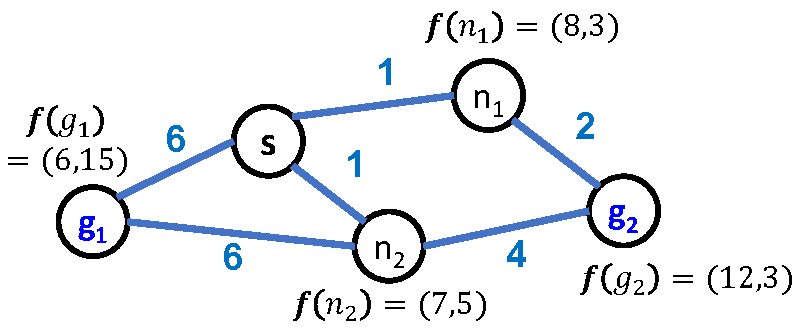
\includegraphics[width=0.9\columnwidth]{need-resort_cropped.pdf}
    \caption{An example where running \kastarmin{} without reordering \open{} after a goal is expanded
        results in expanding redundant states ($n_2$).}
    \label{fig:need-resort}
\end{figure}


Considering stale $F$ values provides poor guidance to the search, directing it
towards goals that are no longer active. For example, consider the \kgs{}
problem depicted in Figure~\ref{fig:need-resort}. The edge weights are depicted
in blue near to the edges. The shortest path to $g_1$ costs of 5, consisting of
following the edge from $s$ to $g_1$, and the shortest path to $g_2$ costs,
going to $g_1$ via $n_1$. After $s$ is expanded there are three states in
\open{}: $g_1$, $n_1$, and $n_2$. Assume that the heuristics $h_1$ and $h_2$
are perfect and therefore we have: $F_{min}(g_1)=\min (6,15)=6$,
$F_{min}(n_1)=\min (8,3)=3$, and $F_{min}(n_2)=\min (7,5)=5$. Thus, $n_1$ is
expanded next, adding $g_2$ to \open{} with $F_{min}(g_2)=\min (12,3)=3$, which
is immediately expanded. At this stage \open{} contains two states: $g_1$ with
$F(g_1)=6$, and $n_2$ with $F(n_2)=5$. So $n_2$ would be expanded, followed by expanding $g_1$ and halting. However, the
$F$ values of $g_1$ and $n_2$ were stale, as they were computed when $g_2$ was
active. Now, imagine that after expanding $g_2$ we
would have re-computed the $F$ values of $n_2$ and $g_1$. Then, their $F$
values would be $F(g_1)=6$ and $F(n_2)=7$, and consequently, $g_1$ would have
been expanded before $n_2$. At this stage the search would halt, returning the
optimal paths to $g_1$ and $g_2$ without ever expanding $n_2$. Indeed, $n_2$ is
a surplus state (Definition~\ref{def:surplus}) with respect to both $g_1$ and
$g_2$. Thus, considering stale $F$ values introduced inefficiency to the
search.

%[[AF: there is a big mess in the exact f-values between the text and the figure. Please correct it.]]

%[[AF: This example is hard to follow. You must to place edge weights in the figure to make it easy. Why is N2 surplus? what are the optimal paths to each state? Give more information. Two sentences start with "Note". Please rewrite and better explain.]]
%The problem is even graver when using \kastarmax{}, where re-computing the $F$ value of some of the states in \open{} is necessary to ensure optimality of the returned paths. For example, consider running \kastarmax{} on the same \kgs{} problem given in Figure~\ref{fig:need-resort}, and assume that all $f$ values are accurate. In this case, $n_2$ will expanded first, followed by $g_2$ and $g_1$ choose from \open{} is $n_1$ with $F(n_1)=5$. and may cause \kastarmin{} to expand states that are surplus for all  for states already generated there is no point in considering the $f$ values for goals that are no longer active, as it will unnecessarily guide the search towards an already achieved goal.





%sec:smart-eager

\subsection{Reordering \open\ eagerly}
\label{sec:eager}
One option to address this is to completely reorder \open{} after removing a
goal from the list of active goals (line~\ref{line:removeGoal}). In other
words, when a goal is expanded, recompute the state evaluation function ({\tt
ComputeF}) for all states in \open{} to get an updated $F$ value and then
reorder \open{} accordingly. We refer to this option as {\em Eager \kastar{}}.
Using Eager \kastar{} can be costly, as it requires reordering \open{} $k-1$
times. We analyze this added overhead in Section~\ref{sec:theoretical-analysis}.


Observe that the $F$ value of some states do not change when reordering \open{}
after a goal is expanded. For example, consider a state $n$ with $F$ value that
is computed from the vector of $f$ values $\textbf{f}(n)=(10,5,3)$. When using
\kastarmin{}, $F(n)=f_3(n)=3$. Therefore, the $F$ value of $n$ will only change
if the goal $g_3$ is expanded and consequently removed from the set of active
goals. Importantly, there is no need to re-compute it after goals $g_1$ or
$g_2$ are selected for expansion. More generally, after a goal $g_i$ is
expanded there is no need to re-compute the $F$ value of any state for which
$F(n)\neq f_i(n)$.

%[[AF: hoe about principal goal? or key goal?]]
We implemented this optimization by keeping track of the {\em responsible goal}
for every state $n$, that is, the goal $g_i$ for which $F(n)=f_i(n)$. If there
are multiple responsible goals, we choose one arbitrarily. [[AF: Why? choose
them all. Only when it is empty you should re-order open]] Then, we only
re-compute the $F$ value of a node if its responsible goal is expanded. This
version of Eager \kastar{} is referred to as Eager$^+$. [[AF: I would not call
it eager+. This is an implementation trick for eager and should not have its
own sign.]] [[AF: you do not only recompute. You also change its place in OPEN.
If there are too many of these, why not sort OPEN from scratch?]]

A more involved implementation would keep track of the set of responsible goals
for every state, i.e., the set of goals for which their $f$ value is equal to
that states $F$ value. Then, when a goal $g_i$ is expanded, we iterate over
every state that had $g_i$ in the set of responsible goals and remove $g_i$
from that state. Then, a state will only re-compute its $F$ value (and reposition it in \open{} accordingly) if its set of
responsible goals is empty. This approach, however, has requires storing more
information per state and is more complex, and so we implemented only Eager$^+$
in our experimental. %[[AF: OK, you answered me. But, I think this should be the correct way to do eager. I do not like eager+ not in its name and not in its content. By the end of the day, the responsible goal is out of the computation so it does not really matter.]]
%former approach, which keeps track of a single responsible goal.

%[[AF: the last sentence is not understandable. you keep the set for who? Which nodes? For everybody? please better explain what you mean. I did not understand. Also, consider to delete this all together. You did not implement it so why bother? Maybe in a footnote? But, please better explain for sure.]]

%[[AF: I would delete all the non eager+ from the experiments]]

% Lazy!

\subsection{Lazy \kastar{}}
% We outlined above an example where the cost of reordering \open{} after a goal is expanded does not [[AF: I think you want to delete the "not"]]incur significant overhead [[AF: where did you outline this? You just showed that you must reorder open, otherwise, you have more node expansions]]. However, this is not always the case. For example, in domains where the search frontier does not grow exponentially, then states generated after the $k-1$ goal has been expanded are not larger than the states generated up to that point. Indeed, we show in our experimental results that in some domains reordering does, in fact, incur a significant amount of runtime.
%[[AF: you just said that it is negligible. Please explain why this is not the case in these domains. Are they polynomial?]]

%[[AF: Roni will reword and say that eager can be costly.]]

Both Eager \kastar{} and Eager$^+$ \kastar{} will re-compute the $F$ value and reorder all the states in \open{} that have stale $F$ values. 
This incurs a cost that can be significant, and indeed we observe this in our experimental evaluation. To this end, we propose an alternative approach in which states are re-evaluated and reordered in a lazy manner. This means that only when a state is popped out of \open{} for expansion (line~\ref{line:open:chooseNode} in
Algorithm~\ref{alg:kastar}), we re-compute its $F$ value.\footnote{Actually, we only consider re-computing the $F$ value of a state if its responsible goal is no longer active.} If its $F$ value has
increased and it is no longer the minimal in \open, we re-insert it into
\open{}. 



We call this algorithm Lazy \kastar{}, since it is directly inspired
by the Lazy \astar{} algorithm~\cite{betzalel2015typeSystem,tolpin2013toward},
where multiple heuristics are used towards the same goal, and are evaluated
lazily in a similar manner. Lazy \kastar{} behaves differently when using
\maxf{} and when using \minf{}. Thus, we analyze them separately.
%[[AF: I already said that I think these terms are redundant. Your call]]\roni{I don't see a better way to discuss the different F functions then to name them}

%n particular, the lazy approach only brings benefit to \kastarmin{}




\begin{figure}
    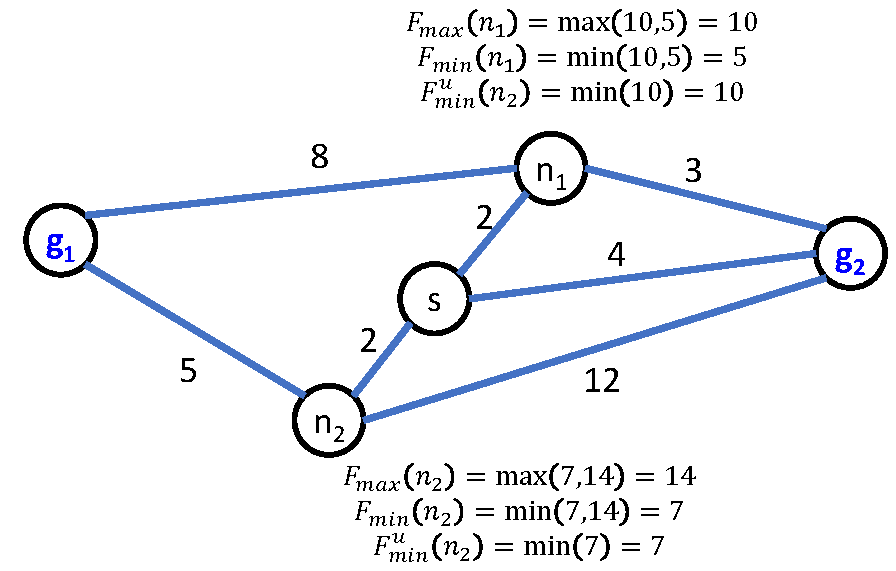
\includegraphics[width=\columnwidth]{Lazy_cropped_cropped.pdf}
    \caption{An example of using Lazy \kastarmin{}.}
    \label{fig:lazy}
\end{figure}



\subsubsection{Lazy \kastarmin{}}

Consider running Lazy \kastarmin{} on the graph depicted in
Figure~\ref{fig:lazy}. Assume we have a perfect heuristic for all states except
for the goal states $g_1$ and $g_2$ that have a zero heuristic to each other,
i.e., $h_2(g_1)=0$ and $h_1(g_2)=0$.
%[[AF: can you give them epsilon heuristic?]] \roni{why?}
After expanding the start state $s$, states $n_1$, $n_2$, and
$g_2$ are generated. Using \minf{}, we have $F(n_1)=\min(10,5)=5$,
$F(n_2)=\min(7,14)=7$, and $F(g_2)=\min(0,0)=0$. So the next state expanded is
goal $g_2$, which is then removed from the set of active goals. At this stage,
states $n_1$ and $n_2$ are both in \open{} and their $F$ values are stale.
% in the sense that they were computed for $g_1$ and $g_2$ while the set of active goals at this stage contain only $g_2$ [[roni: already defined above]]
According to these stale $F$ values, the next state to
choose from \open{} is $n_1$ with $F(n_1)=5$. After selecting $n_1$ for expansion from
\open{}, its $F$-value is re-computed using Lazy \kastar{}. We denote
by $F^u_{min}(n_1)$ this updated $F$-value of $n_1$, which is computed with respect
to the current set of active goals. According to Lazy \kastar{}, if
$F^u_{min}(n_1)> F(n_1)$ then we set $F(n_1)$ to be $F^u_{min}(n_1)$ and re-insert
$n_1$ into \open{}. Consequently, $n_2$ will be expanded, followed by $g_1$,
finally completing the search with an optimal path to both goals. %$g_1$ as well.







We now prove that although Lazy \kastarmin{} does not reorder all the states in
\open{} when a goal is expanded, it still expands states in order of their
up-to-date $F$ values (i.e., according to the $F^u$ value).
% Lazy with minf is good
\begin{lemma}[The Efficiency of Lazy \kastarmin{}]
Lazy \kastarmin{} always expands the state in \open{} with the smallest $F^u$
%Every path $\pi_i$ returned by Lazy \kastarmin{} is guaranteed to be the lowest-cost path to its corresponding goal ($g_i$).
\label{the:lazy-minf-correct}
\end{lemma}
\begin{proof}

%[[AF: the same sentence is repeated three times.]]

We prove Theorem~\ref{the:lazy-minf-correct} by induction on the iterations of
the main loop of Lazy \kastarmin{}.
%, showing that Lazy \kastarmin{} and Eager \kastarmin{} expand exactly the same set of states.
The base of the induction is trivial: in the first step $F(s)=F_u(s)$. Now assume that in the first $m-1$ iterations, Lazy \kastarmin{} expanded the state with the smallest $F^u$ value, and consider the $m^{th}$ iteration of Lazy \kastarmin{}.
%  up to tie-breaking [[AF: what do you mean up to tie breaking. If you break ties differently, it is not the same set of states. So, how can you prove it? Maybe say that we assume that they break ties in the same manner?]], and consider the $m^{th}$ iteration of Lazy \kastarmin{}.


First, observe that for every state $n$, the value $F_{min}(n)$ is the minimum
over the heuristic values computed for the old set of active goals, while
$F_{min}^u(n)$ is the minimum over the heuristic values computed for the current
set of active goals. Since the old set of active goals is a superset of the
current set of active goals then for every $n$ it holds that $F_{min}(n)\leq
F^u_{min}(n)$.
%This is true because $F_, since $F^u_{min}(n)$ is the minimum over a subset of elements that $F_{min}(n)$ is a minimum of.
Now, let $n$ be the state selected fro expansion from \open{} in the $m^{th}$
iteration of Lazy \kastarmin{}. Hence, it had the smallest $F$-value in
\open{}. In addition, $F_{min}(n)=F^u_{min}(n)$, as otherwise it would have
been re-inserted into \open{}. Therefore
\[ \forall n'\in\open{} ~~ F^u_{min}(n)=F_{min}(n)\leq F_{min}(n') \leq F^u_{min}(n') \]
    So, $n$ has the smallest $F^u_{min}$ value in \open{}, as required.
\end{proof}

The implication of Lemma~\ref{the:lazy-minf-correct} is that both Lazy
\kastarmin{} and Eager \kastarmin{} expand states according to their $F^u$
values, except that Lazy \kastarmin{} does so more efficiently, without the
need to reorder all the stale states in \open{}. 
% [[AF: So you do reorder the entire open list. with Eager. Or do you only insert these nodes that their F values was changed?]]
However, the exact set of states they expand may be different
due to tie breaking. For example, consider a tie-breaking rule that prioritizes
states for which the sum of their $f$ values is smaller, and assume we have two
states in \open{}, $n_1$ and $n_2$, with $\mathbf{f}$ values (5,6,10) and
(5,7,7), respectively. They have the same \minf{} values (5), but according to
this tie-breaking rule \kastarmin{} will chose $n_2$ before $n_1$. Now, assume
that $g_3$ was expanded. Using Eager \kastarmin{} would result in $n_1$ now
being expanded before $n_2$, while Lazy \kastarmin{} would not do so. Since
tie-breaking rules can be useful in practice, this means that Eager
\kastarmin{} may still outperform Lazy \kastarmin{}. In our experimental
results, however, this did not occur and Lazy \kastarmin{} was in general
better. %[[AF: Tie breaking can go either way. You might want to delete all this altogether]]\roni{I don't follow}


% Lazy does not work for Max-f, but does work on Min-f
\subsubsection{Lazy \kastarmax{}}

%Using Lazy \kastarmin{} has significant impact [[AF: what do you mean, runs faster? explain why?]] in practice. Unfortunately,
Lemma~\ref{the:lazy-minf-correct} does not transfer to Lazy \kastarmax{}.
%Using the Lazy approach for \kastarmax{} does not have the same effect.
In fact, we show next that Lazy \kastarmax{} expands
the same states as \kastarmax{} without reordering \open{} after a goal is expanded,
and thus it may expand states that do not have the lowest updated $F$ value in \open{}.
%[[AF: who is not doing the reordering. Ambiguous. Please precisely say what you mean]].
%[[AF: recall? I do not remember anything??]]
As discussed above (and shown in the example in Figure~\ref{fig:need-resort}), this is a negative
result since it means that Lazy \kastarmax{} will be guided towards goals even
after the optimal path to them has been found.
% were already solved. %misinformed heuristics. % we cannot apply the lazy approach to \kastarmax{} and preserve admissibility.
\begin{theorem}[Lazy \kastarmax{} is Ineffective]
Lazy \kastarmax{} expands exactly the same set of states as \kastarmax{},
without reordering \open{}.
    \label{the:lazy-maxf-bad}
\end{theorem}
\begin{proof}
    To prove Theorem~\ref{the:lazy-maxf-bad}, we show that Lazy \kastarmax{} never decides to re-insert the state it chooses from \open{}. Let $n$ be a state with the minimal $F$ value in \open.
    For Lazy \kastar{} to decide to re-insert $n$,  its $F$ value must be stale and after updating its $F$ value
    (from $F(n)$ to $F^u(n)$) then it will not have  the minimal $F$ value in \open{}.
    We show now that this cannot occur. %below [[AF: you mean right now]]
    Let $A$ be the set of active goals when
    $n$ was expanded, and let $A^u$ be the current set of active goals. Clearly, $A\subseteq A^u$.
    In \kastarmax{}, we have that $F(n)=$\maxf{}, which is the maximum of the heuristics for the active goals.
    Thus, $F^u(n)=\max_{i\in A^u} h_i(n)\leq \max_{i\in A} h_i(n) = F(n)$.
\end{proof}
%Consider Figure~\ref{fig:lazy}(a). First $s$ is expanded, generating $n_1$ and $n_2$ with ${\textbf{f}}(n_1)=(10,3)$  and ${\textbf{f}}(n_2)=(7,7)$. Thus, $n_2$ will be expanded, generating $g_1$ and $g_2$, each with a $g$ value of 7.  Assume that the heuristic of $g_1$ and $g_2$ are both zero (for both goals). Then \kastarmax{} will expand next $g_1$ and $g_2$, never expanding $n_1$ and returning a suboptimal path to $g_2$ of cost 7.

% Using Lazy \kastarmin{} has significant impact in practice, as it decides in many cases to re-insert into \open{} the state with the minimal $F$ value. This is not the case in Lazy \kastarmax{}. In fact, Lazy \kastarmax{} will {\em never} re-insert a state into \open{} after re-computing its $F$ value.
%To better understand why Lazy \kastarmax{} This is because re-computing an $F$ value for a state after the set of relevant goals has been reduced will only cause the $F$ value to decrease. Thus, is a state already has the smallest $F$ value in \open{}, it will still have the smallest $F$ value after we re-compute its $F$ value.
For the above reason, we only implemented for \kastarmax{} the two Eager approaches (Eager and Eager$^+$).

%[[AF: not clear. You never used lazy? What two approaches. This entire section needs some more rewording as I said. I think I do want to see this section 5 again.]]

%[[AF:  As I said above, I think we only need eager and the exact implementation is less important. That is, I do not like the term eager+. Your call]]

\section{Theoretical Analysis}
\label{sec:theoretical-analysis}
% Analysis

In this section we compare analytically the two main approaches we proposed for
the \kgs{} problem: $k$ searches for one goal (\kxastar{}) or one search for
$k$-goals (\kastar{}).

\subsection{Expanded States}
\label{sec:expandedStates}
First, we analyze the set of states expanded by the two approaches.
Let \astari{i} denote   the \astar{} search used to solve $\Pi_i$ (the SSP problem of finding a path to goal $g_i$).
We denote by Exp(\astari{i}), Exp(\kxastar{}), Exp(\kastarmin), and Exp(\kastarmax),
the set of states expanded by \astari{i} (for a given $i$), \kxastar{}, \kastarmin, and \kastarmax{}, respectively.
It is easy to see that
\[ Exp(\text{\kxastar{}})=\cup_{i=1}^k Exp(\text{\astari{i}}) \]
Note that Exp($X$) is the {\em set} of states that were expanded, and not the number of state expansions, i.e., if a state is expanded twice then it will only exists once in Exp($X$).


To analyze the relationship between Exp(\kxastar{}), Exp(\kastarmin), and Exp(\kastarmax), we expand the notion of surplus and surely necessary states (Definitino~\ref{def:surplus}) to the \kgs{} problem setting.
\begin{definition}[Surplus and Surely Necessary in \kgs{}]
    A state is {\bf surely necessary} with respect to a \kgs{} problem
    if it is surely necessary for {\bf at least one} of the SSP problems $\Pi_1,\ldots, \Pi_k$.
    A state is {\bf surplus} with respect to a \kgs{} problem
    if it is a surplus state for {\bf all} SSP problems $\Pi_1,\ldots, \Pi_k$.
    $\tuple{G,s, \textbf{g}}$
\label{def:surplus-k-goal}
\end{definition}
By definition, \kxastar{} never expands any surplus states and always expands
all surely necessary states.


\begin{theorem}
    For a given \kgs{} problem, Eager \kastarmin{} never expands any surlpus states and
    expand all the surely necessary states.
    \label{the:kastarmin-effective}
\end{theorem}
\begin{proof}
{\bf No surplus states.}    We prove Theorem~\ref{the:kastarmin-effective} by showing that every state $n$
    expanded by \kastarmin{} there exists $i\in [1,k]$ for which $f_i(n)\leq opt_{\Pi_i}$.
    By negation, if this does not hold for $n$, then $\forall i\in[1,k]~f_i(n)>opt_{\Pi_i}$.
    Since $n$ has the smallest $F$ value in \open{} and we are using \minf{}, then
    for every other state $n'$ in \open{} it also hold that $\forall i\in[1,k]~f_i(n')>opt_{\Pi_i}$.
    Thus, there is no state that in on an optimal path to any of the goals, contradicting Lemma~\ref{lem:simple}. \\

    {\bf All surely necessary states.} Again, we prove this by negation. Let $n$ be a state
    that is surely necessary for goal $g_i$ but was not expanded by \kastarmin{}.
    That is, $n$ is reachable from $s$ by a path of states with $f_i$  values lower than $opt_{\Pi_i}$
    and $f_i(n)<opt_{\Pi_i}$. The $F$ values of the states along this path must also be lower than
$opt_{\Pi_i}$ (since we are using \minf). Since all edges in the underlying
graph are non-negative, then $F(g_i)=opt_{\Pi_i}$. Hence, the minimal $F$ value in \open{} is $opt_{\Pi_i}$ when $g_i$ is expanded. Thus, all the states along the path to $n$ and $n$ itself must have already been expanded, as all of them have $f_i$ values smaller than $opt_{\Pi_i}$ and thus also have $F$ values smaller than $opt_{\Pi_i}=F(g_i)$.  
\end{proof}

An equivalent theorem for \kastarmax{} does not exists. In fact, there are
cases where \kastarmax{} indeed expands surplus states. For example, consider
the \kgs{} problem in Figure~\ref{fig:need-resort}. State $n_2$ will be
expanded first, having $F_{max}(n_2)=7$, followed by $n_1$ ($F_{max}(n_1)=8$),
$g_2$ ($F_{max}(g_2)=12$), and finally $g_2$ ($F_{max}(g_1)=15$). However,
neither \astari{1} nor \astari{2} will expand $n_2$. Moreover, $n_2$ is surplus
w.r.t both $\Pi_1$ and $\Pi_2$, since the optimal path to $g_1$ and $g_2$ costs
6 and 3, respectively, while $f_1(n_2)=7>6$ and $f_1(n_2)=5>3$.


The practical implication of Theorem~\ref{the:kastarmin-effective} is that, up
to tie breaking, \kastarmin{} and \kxastar{} expand the same set of states.
More formally, assume that both \kastarmin{} and \kxastar{} use the same
tie-breaking function to choose which state to expand among the states with the
same $F$ and $f$ value, respectively. [[AF: they have different knowledge, how
can they practically use the same order unless they do not look on f-values but
only look on the description of the state]] A tie-breaking function induces a
total order between states. Let $\prec$ denote the total order induced by the
tie-breaking function used by both \kastarmin{} and \kxastar{}. Under these
assumption, the following theorem holds.

\begin{theorem}
    If the tie-breaking function used by Eager \kastarmin{} and \kxastar{}
    induce the same total order over states then
    \[Exp(\text{\kastarmin{}})=Exp(\text{\kxastar{}}) \]
    \label{the:expanded-equal}
\end{theorem}
\begin{proof}
    Let \open$_{X,t}$ denote the open list of algorithm $X$ at iteration $t$. 
    By negation, let $t$ be the first \kastarmin{} iteration in which it expands
    a state that is not expanded by any of the $k$ individual \astar{}s, and let $n$ be that state. This means that there exists $t_1,\ldots,t_k$ such that before expanding $n$
    \begin{equation}
    \open{}_{\text{\kastarmin{}}}=\bigcup_{i=1}^k \open_{\text{\astari{i}},t_i}
    \label{eq:union-of-open}
    \end{equation}
    That is, since until this iteration \kastarmin{} only expanded states 
    that were expanded by at least one of the individual \astar{}s then 
    $\open{}_{\text{\kastarmin{}}}$ is the union of the open lists of the individual \astar{}s
    at some iteration of their search. 
    Since $n$ was selected for expansion, it has the minimal $F_{min}$ value
in \open{}$_{\text{\kastarmin{}}}$. Let $g_i$ be the responsible goal for $n$,
i.e., a goal for which $f_i(n)=F_{min}(n)$.
Since we assume that $n$ was not expanded by any of the $k$
\astar{} searches, it must have also not been expanded by \astari{i}.
This means there exists $n'\in\open_{\text{\astari{i}},t_i}$ for which either $f_i(n')<f_i(n)$
or $n'\prec n$. Due to Equation~\ref{eq:union-of-open}, we have that $n'$ is in \open{}$_{\text{\kastarmin{}}}$,
and therefore neither of these conditions can hold, or else $n'$ was selected for expansion before $n$. Thus, \astari{i} must have expanded $n$ at iteration $t_i$
\end{proof}
Note that while every tie-breaking function used by the individual \astar{} searches 
can be trivially applied in \kastarmin{}, the reverse is not necessarily true. In fact, \kastarmin{} may employ a tie-breaking mechanism that is more informed 
than those used by the individual \astar{} searches, as it has more knowledge about the overall \kgs{} problem. 


% Memory=generated
\subsection{Memory Requirements}
The number of states expanded is directly related to the number of generated
states,\footnote{If $b$ is the branching factor then there are $b$ times
more generated states than expanded states.} which in turn is related to the
memory requirements of \astar{} and \kastar{}. In general, search algorithms
that store all the generated states in \open{} and in \closed{}, such as
\astar{} and \kastar{}, are memory intensive. While other implementations are
also possible, where only the states in \open{} and their predecessors are
stored~\cite{zhou2006breadth,korf2004best} or where the states are stored in
external
memory~\cite{zhou2004structured,edelkamp2016external,edelkamp2005external}, we
focus our analysis on the more common implementation of \astar{} in which all
generated states are stored in memory for the entire duration of the search.

Hence, the memory required for the algorithms discussed in this paper
proportional to the number of (distinct) states generated times the memory
required to store a single state.
%Without loss of generality, assume that each state requires one memory units to store and denote by Gen($X$) the set of states generated by algorithm $X$. From Observation~\ref{obs:expandedStates}, we can bound the memory required to run \kastarmin{} as follows:
In our analysis we make the simplifying assumption that each state requires one
memory unit to store for all algorithms.\footnote{This assumption is not
exactly correct in practice, since in \kastar{} we store for a state a vector
of $k$ values ($\textbf{f}(n)=(f_1,\ldots,f_k)$)  while in \astar{} we only
store a single value. Nonetheless, we justify our assumption for cases where
the memory required to store the state details is significantly larger than
these $k$ values.} Hence, if Mem($X$) and Gen($X$) denotes the memory required
and the set of states generated when running algorithm $X$, respectively, then,
up to tie-breaking between states with the same $F$ value, it holds that:
\begin{align}
Mem(\text{\kxastar{}})&=\max_{j\in [1,k]}| Gen(\text{\astari{j}})| \label{eq:kxastar-mem}\\
Mem(\text{\kastarmin{}})&=|\bigcup_{j\in [1,k]} Gen(\text{\astari{j}})| \label{eq:kastar-mem}\\
Mem(\text{\kxastar{}})&\leq Mem(\text{\kastarmin{}}) \leq \sum_{j\in[1,k]} Mem(\text{\astari{j}}) \label{eq:kxastar-kastar-mem}
\end{align}

The correctness of Equations~\ref{eq:kxastar-mem}-\ref{eq:kxastar-kastar-mem}
is now established. Since \kxastar{} runs the $k$ searches individually, there
is no need to store the states generated by \astari{i} when running \astari{j}.
Thus, to run \kxastar{} we require memory sufficient to run each \astari{i}
individually (Equation~\ref{eq:kxastar-mem}). In \kastarmin{} we expand the
same set of states as \kxastar{} and thus generate the same set of states, but
we must store them throughout the search. Thus, \kastar{} stores every state
$n$ that is  generated by one of the $k$ searches in \kxastar{}, i.e., the
union $\bigcup_{j\in[1,k}Gen(\text{\astari{j}})$
(Equation~\ref{eq:kastar-mem}). The size of this union cannot be smaller than
the cardinality of the set of stated generated by any individual \astar{}, but
cannot be larger than their sum (Equations~\ref{eq:kxastar-kastar-mem}). Note
that these bounds are tight, in the sense that there are $k$-goal problems
where $Mem(\text{\kxastar{}}) = Mem(\text{\kastarmin{}})$ and other $k$-goal
problems where $Mem(\text{\kastarmin{}}) = \sum_{j\in[1,k]}
Mem(\text{\astari{j}})$. For example, in a 2-goal instance, if
$Gen(\text{\astari{1}})\subset Gen(\text{\astari{2}})$ then
$Mem(\text{\kxastar{}}) = Mem(\text{\kastarmin{}})$ while if
$Gen(\text{\astari{1}})\cap Gen(\text{\astari{2}})=\{s\}$ then
$Mem(\text{\kastarmin{}}) = \sum_{j\in[1,k]} Mem(\text{\astari{j}})-1$, 
where the minus one is for the start state. %[[AF:Except for the start state]]

\subsection{Runtime Analysis}

Now we analyze the expected runtime of the proposed \kgs{} algorithms. As shown
above theoretically and will be shown later experimentally, \kastarmin{} is
almost always superior to \kastarmax{}, and thus the focus of our analysis is a
comparison between \kxastar{} and \kastarmin{} (denoting the latter as simply
\kastar{} throughout this section).  While both algorithms generate the same
set of states (Theorem~\ref{the:expanded-equal}), their runtime differ due to the number of times each state is
generated and the cost of these generations.



%%%%%%%%%%%%%%%%%%%%%%%%%%%%%
\subsubsection{Runtime of \kxastar{}}
To analyze the runtime of \kxastar{}, consider the operations performed by an \astar{} search whenever a state is generated (lines~\ref{line:astar:generate-start}-\ref{line:astar:generate-end} in
Algorithm~\ref{alg:astar}):

\begin{enumerate}
    \item {\bf Generation}  (lines~\ref{line:astar:generate-start}-\ref{line:dd-end} and \ref{line:astar:generate-end}).
    This refers to computing the generated state by applying an action to the expanded state,
    performing duplicate detection (updating the $g$ value to the generated if needed),
    and inserting the generated state to \open{} (if needed).
    We denote the computational cost of this step as $C_{gen}$.


    \item {\bf Heuristic computation}  (line~\ref{line:compute-f}). This refers to computing the $h$ value of the generated state.
    We denote the computational cost of this step as $C_{h}$.
\end{enumerate}

The exact value of $C_{gen}$ depends on the domain and various implementation
details, such as the data structure used to implement \open{} and the state
representation. In the textbook implementation of \astar{} on simple domains,
\open{} is implemented as a Binary heap and the domain actions are easy to
compute and so $C_{gen}$ is linear in the size  of a state's representation in
memory and (plus) logarithmic in the size of \open{} (the cost of inserting an
item in a Binary heap). But faster implementations are also possible in some
domains, where adding to \open{} incurs a constant
time~\cite{GILON2016,BurnsHLR12}. Similarly, the cost of the heuristic
computation ($C_h$) can vary widely as well, where some heuristics require
constant time to compute while more sophisticated heuristics may involve
poly-time computations or even worse.


%Each of these operations incur some computational cost. Let $C_{gen}, C_{dd}, C_{h},$ and $C_{add}$ denote the average computation cost of the above four operations, generation, duplicate detection, heuristic computation, and insertion into \open{}, respectively. In addition,

%[[AF: either the i is a subscript or in brackets. Standardize.]]
We perform our runtime analysis with respect to the above cost model,
which assumes that $C_{gen}$ and $C_h$ are approximately constant
for all states. Under this assumption, the runtime of \kxastar{} is straightforward.
\[
Time(\text{\kxastar{}}) = \sum_{i\in[1,k]} |Gen(\text{\astari{i}})|\cdot (C_{gen}+C_h)
\]
where Time($X$) denote the runtime of algorithm $X$.

\subsubsection{Runtime of \kastar{}}

To analyze the runtime of \kastar{}, a deeper analysis is needed. In addition
to node generation ($C_{gen}$) and heuristic computation ($C_h$), in \kastar{}
we also have the cost of reordering \open\ (either Eagerly or Lazily), which
incurs $C_r$ for every state in \open{}. Next, we consider the number of times
each of the costs components -- node generation ($C_{gen}$), heuristic
computation ($C_h$), and state reordering ($C_r$) -- is incurred.

\noindent {\bf Node generation} ($C_{gen}$). Every generated state incurs
$C_{gen}$ exactly once. Thus, state generation contributes to the overall runtime of \kastarmin{}:
\[
|Gen(\text{\kastar{}})|\cdot C_{gen} =
|\bigcup_{i\in{\{1,k\}}} Gen(\text{\astari{i}})|\cdot C_{gen}
  \displaystyle
\]
\noindent {\bf Heuristic computation} ($C_{h}$). 
Let $Gen_i(\text{\kastar{}})$ denote the set of states generated by \kastar{} until goal $g_i$ is expanded. 
Until the first goal is
expanded, \kastar{} computes $k$ heuristics. Then, until the second is
expanded, \kastar{} computes $k-1$ heuristics, and so on. 
So, $|Gen_1(\text{\kastar{}})|$ states are generated with
$k$ heuristics, 
$|Gen_2(\text{\kastar{}})|-|Gen_1(\text{\kastar{}})|$ states are generated with $k-1$
heuristics, $|Gen_3(\text{\kastar{}})|-|Gen_2(\text{\kastar{}})|$ states are generated with $k-2$
heuristics, and so on. Summing all this, we have that 
heuristic computations add to the overall runtime of \kastarmin{}:
\begin{align*}
    C_h\cdot ( k \cdot & (|Gen_1(\text{\kastar{}})| \\
     + (k-1) \cdot&(|Gen_2(\text{\kastar{}})|-|Gen_1(\text{\kastar{}})|)\\
     + (k-2) \cdot&(|Gen_3(\text{\kastar{}})|-|Gen_2(\text{\kastar{}})|) \\
     &\ldots\\
     %+ 2 \cdot&(|Gen_k(k-1)|-|Gen_k(k-2)|) \\
     + 1 \cdot&(|Gen_k(\text{\kastar{}})|-|Gen_{k-1}(\text{\kastar{}})|)))\\
     =& C_h \cdot \sum_{i\in[1,k]} |Gen_i(\text{\kastar{}})|
\end{align*}

%\[=\sum_{i\in[1,k]} |Gen_k(i)|\cdot C_h\]
%So, Gen_k(1) states are generated with $k$ heuristics, $Gen_{k}(2)$ states with $k-1$ heuristics,a nd so on. Summing all this, we have that in \kastarmin{}, heuristic computations add to the overall runtime:
%\[ \sum_{i\in[1,k]} Gen_k(i)\cdot C_h \]




\noindent {\bf Reordering of \open{}} ($C_r$).
%\open{} gets reordered after every goal is found (except for the last goal).

It is difficult to exactly analyze the runtime incurred due to these reordering
operations performed by the \kastar{} variants (Eager, Eager$^+$, and Lazy).
Thus, we perform here only a rough analysis of the overhead incurred by
reordering \open{} in Eager \kastarmin{}. This is intended to serves as an
upper bound approximation of the reordering overhead of Eager$^+$ and Lazy
\kastarmin{}.


Let $\open{}_i(X)$ denote the number of states in \open{} when algorithm $X$
expanded goal $g_i$, and let $C_r$ be the cost of re-computing the $F$ value
(using either \minf{} or \maxf{}) for a state and updating its position in
\open{} accordingly. Without loss of generality, assume that $g_i$ is the
$i^{th}$ goal that has been found. After $g_i$ was expanded, there are
$\open{}_i(\text{\kastar{}})$ states in \open{}. Thus, the total computational
cost incurred by Eager \kastar{} due to recomputing $F$ values and reordering
\open{} accordingly after expanding  all the goals is
\begin{equation}
C_{eager}=\sum_{i=1}^{k-1} \open{}_i(\text{\kastar{}}) \cdot C_r
\label{eq:re-sort-cost}
\end{equation}


\subsubsection{Practical Implications}
To show the usefulness of the above runtime analysis, we  consider some special
cases, e.g.,  where one of the costs ($C_{gen}$, $C_{h}$, and $C_{r}$) dominates others:
\begin{itemize}
    \item {\bf Case 1: State generation cost is dominant.} ($C_{gen}>>C_{h}+C_r$)
    If this case, the preferred algorithm is \kastar{}. To show this,
    compare the values in Table~\ref{tab:time-analysis} for $C_{gen}$: $\sum_{i\in[1,k]} |Gen(\text{\astari{i}})|$
    versus $|\bigcup_{i\in[1,k]} Gen(\text{\astari{i}})|$. Clearly, the former is larger than or equal to the latter.
    The advantage of \kastarmin{} grows with the size of the intersection between the sets $Gen(\text{\astari{i}})$ for $i\in[1,k]$.

    \item {\bf Case 2: Heuristic computation is dominant.} ($C_{h}>>C_{gen}+C_r$)
    If this is the case, the preferred algorithm is \kxastar{}. Again, to show this we look at
     Table~\ref{tab:time-analysis} and see that \kxastar{} computes a heuristic function
    $\sum_{i\in[1,k]} |Gen(\text{\astari{i}})|$ times, while
    \kastar{} computes the heuristic $\sum_{i\in[1,k]} |Gen_i(\text{\kastar})|$ times.
    Importantly, for every $i$ it holds that $|Gen_i(\text{\kastar})|\geq |Gen(\text{\astari{i}})|$
    because $Gen_i(\text{\kastar})$ contains all the states in $Gen(\text{\astari{i}})$
    and states associated with the search for the other goals
    (those states that \astari{i} would not generate but some of other individual \astar{} searches would) that happen to have been added to \open{} at this stage.

   \item {\bf Case 3: Distant Goals.} ($|\bigcap_{i\in[1,k] Gen(\text{\astari{i}})}|\approx 1$)
   If the goals are far away from each other in the state space,
   then we expect most states to be generated by only one of the $k$ searches.
   In such a case, $\sum_{i\in[1,k]}|Gen(\text{\astari{i}})|\approx |\bigcup\limits_{i\in[1,k]} Gen(\text{\astari{i}})|$
   and therefore we expect \kastar{} to be less effective.
\end{itemize}




\begin{table}
	\begin{tabular}{|l|l|l|}
		\hline
		Cost        & \kxastar{}                                    & \kastarmin \\ \hline
		$C_{gen}$   & $\sum\limits_{i\in[1,k]} |Gen(\text{\astari{i}})|$       & \newcode{$|\bigcup\limits_{i\in[1,k]} Gen(\text{\astari{i}})|$}\\
		$C_{h}$     & \newcode{$\sum\limits_{i\in[1,k]} |Gen(\text{\astari{i}})|$}    & $\sum\limits_{i\in[1,k]} |Gen_i(\text{\kastar{}})|$\\
		$C_r$       & \newcode{0}                                               & $\sum_{i=1}^{k-1} \open{}_i(\text{\kastar{}}) \cdot C_r$\\
		\hline
	\end{tabular}
	\caption{Analysis of the computational costs incurred by \kxastar{} and \kastarmin{}.}
	% when solving a \kgs{} problem with arbitrary $k$.  Some costs are incurred the same or less in one algorithm than the other. Such cases are marked with an asterisk.}
	\label{tab:time-analysis}
\end{table}


Table~\ref{tab:time-analysis} provides a summary of our runtime analysis, comparing the
runtimes of \kxastar{} and \kastarmin{}. Each row represents one of the
computational costs factors ($C_{gen}$, $C_{h}$, and $C_{r}$), showing the
contribution of that computational cost factor to the overall runtime for the
compared algorithms. 
We highlight the smaller value in each row by coloring it in blue and adding a ``[+]'' sign. This is intended to provide a higher-level view of the outcome of our analysis: if one of the costs factors is particularly high then the algorithm that minimizes the times this cost is incurred is expected to be faster. %algorithm that [[AF: why do you have stars inside the figure. Do you wantto delete them?]]

%We denote this extra cost by $C_{eager}$.  $C_{eager}$ can be negligible compared to the overall runtime of \kastar{}.  For example, consider \kgs{} problems where the goals are not very close to each other  and the frontier of the search grows exponentially.  In such cases, the number of states generated after the $k-1$ goal is expanded  is larger than the number of states generated before that.  Now, observe that every state generated by \kastar{} incurs a computational cost of $C_{gen}$,  which is larger than $C_r$ because $C_{gen}$ includes the costs of  computing the $F$ value and inserting into \open{} like $C_r$, and also the costs  costs of creating the data-structure for representing the generated state and performing duplicate detection.  Thus, in such cases the overhead of reordering \open{} after each of the $k-1$ goals have been expanded, is negligible. Put more formally, let $Gen_i(\text{\kastar{}})$ to denote the set of states generated by \kastar{} until goal $g_i$ is expanded. Since the search frontier grows exponentially,  $\sum_{i=1}^{k-1}|Gen_i(\text{\kastar{}})|<|Gen_k(\text{\kastar{}})|$. Clearly,  $\open{}_i(\text{\kastar{}})<|Gen_i(\text{\kastar{}})|$ and as we explained above $C_r<C_{gen}$,  and so $C_{eager}<|Gen_k(\text{\kastar{}})|\cdot C_{gen}$. The runtime of \kastar{} consists of generating all the states in the search and performing other operations, and so $C_{eager}$ is smaller. See a more detailed analysis of the runtime of \kastar{} in Section~\ref{sec:theoretical-analysis}.

%\roni{Do we need the 2-goal illustration? I have text for it in the drafts.tex [[AF: The two goal illustration will help a lot. I am for it. I almost started doing it myself but if you have it, add it} [[AF: This  $Gen_k(i)$ is a term that no one knows what it is. Can we simplifies it]] \roni{Revised. See if clearer} [[Ariel up to here]]

\section{Experimental Results}

%In this section we compared empirically the performance of the four \kgs{} algorithms we discussed: $k$ \astar{} searches (Section~\ref{sec:k-one-goal}), two versions of \kastar{} (Section~\ref{sec:one-k-goal-search}): \kastarmax{} and \kastarmin{}, and Lazy \kastar{} with \minf{} (Section~\ref{sec:lazy}). We also compared these heuristic search algorithms with uniform cost search.

In this section we compare empirically the performance of the four \kgs{}
algorithms we discussed: \kxastar{} (Section~\ref{sec:k-one-goal}),
\kastarmax{} (Eager and Eager$^+$) and
\kastarmin{}(Section~\ref{sec:one-k-goal-search}) (Eager, Eager$^+$ and Lazy).
A fifth algorithm is {\em uniform cost search} (UCS) (also known as Dijkstra's
algorithm) which is a best first search without a heuristic, i.e., it
prioritize nodes based on their $g$ values only.


We evaluated these algorithms on two domains: the pancake puzzle and path
finding in grids from the Dragon Age video game from the movingai
repository~\cite{sturtevant2012benchmarks}. These two domains represent
different types of search problems. The pancake puzzle is an {\em exponential
domain}, i.e., the state space graph grows exponentially with the depth of the
search and is given implicitly by a start state and a set of state transition
operators. The grid pathfinding domain is a {\em polynomial domain}, i.e., the
entire state space graph is given as input. %, and so the runtime of a single path finding search is polynomial in the problem input (the graph).

%\roni{Meir, please add here details about the maps: which map did you use, etc.}
\subsection{Grid Path Finding}
%\roni{Meir: what was the heuristic used? how were the states generated? how many instances?}


In the following experiment we used the 8-connected {\tt ost001d} grid path
finding map from the the movingai repository~\cite{sturtevant2012benchmarks},
which has approximately 10,500 grid cells. As a heuristic we experimented with
the Octile distance heuristic and the Differential
Heuristic~\cite{goldberg2005computing,ng2002predicting,sturtevant2009memory}.
We focus first on the experiments performed with the simpler Octile heuristic.

\subsubsection{The Impact of Varying the Number of Goals}


\begin{table}[]
    \centering
    \resizebox{\columnwidth}{!}{%
        \begin{tabular}{|r|r|r|rr|rrr|}
            \hline
            &        &                 & \multicolumn{2}{c|}{\kastarmax} & \multicolumn{3}{c|}{\kastarmin}                  \\
            k   & UCS    & \kxastar    & Eager            & Eager$^+$     & Eager           & Eager$^+$     & Lazy            \\
            \hline
            %1   & 41,122 & \textbf{13,987} & \textbf{13,987}  & \textbf{13,987} & \textbf{13,987} & \textbf{13,987} & \textbf{13,987} \\
            2   & 53,583 & 27,389          & 29,286           & 29,286          & 21,686          & 21,686          & \textbf{21,682} \\
            4   & 62,826 & 52,375          & 43,291           & 43,291          & 28,424          & 28,424          & \textbf{28,413} \\
            8   & 68,505 & 101,103         & 55,652           & 55,652          & 36,673          & 36,673          & \textbf{36,650} \\
            16  & 72,196 & 202,715         & 64,805           & 64,805          & \textbf{43,531} & \textbf{43,531} & 43,489          \\
            32  & 74,618 & 407,221         & 70,519           & 70,519          & 49,732          & 49,733          & \textbf{49,662} \\
            64  & 75,998 & 823,018         & 73,841           & 73,841          & 54,357          & 54,355          & \textbf{54,239} \\
            128 & 76,495 & 1,613,628       & 75,341           & 75,341          & 57,932          & 57,930          & \textbf{57,739}\\
            \hline
        \end{tabular}
    }
    \caption{The number of states generated when solving \kgs{} problems with different number of goals ($k$) on the grid pathfinding domain. Highlighted in bold are the best results for every $k$.}
    \label{tab:pathfinding-generated}
\end{table}


\begin{table}[]
    \centering
    \resizebox{\columnwidth}{!}{%
        \begin{tabular}{|r|r|r|rr|rrr|}
            \hline
            &        &                 & \multicolumn{2}{c|}{\kastarmax} & \multicolumn{3}{c|}{\kastarmin}                  \\
            k   & UCS    & \kxastar    & Eager            & Eager$^+$     & Eager           & Eager$^+$     & Lazy            \\
            \hline
            %1              & 3.39 & \textbf{1.86}         & 1.90         & 1.89        & 1.90  & 1.89        & 1.98  \\
            2              & 4.44 & 3.66         & 3.89         & 3.85        & 3.07  & \textbf{3.03}        & 3.04  \\
            4              & 5.09 & 7.07         & 5.79         & 5.68        & 4.09  & 4.17        & \textbf{4.07}  \\
            8              & 5.62 & 13.55        & 7.32         & 7.18        & \textbf{5.43}  & 5.56        & 5.44  \\
            16             & 5.92 & 27.28        & 9.11         & 8.79        & 7.31  & 7.20        & \textbf{6.98}  \\
            32             & \textbf{6.15} & 54.45        & 10.99        & 10.13       & 10.56 & 9.82        & 9.01  \\
            64             & \textbf{6.37} & 111.58       & 15.18        & 11.81       & 19.45 & 14.27       & 12.54 \\
            128            & \textbf{6.68} & 216.28       & 27.02        & 15.06       & 51.83 & 25.29       & 20.49\\
            \hline
        \end{tabular}
    }
    \caption{The runtime in milliseconds for solving \kgs{} problems with different number of goals ($k$) on the grid pathfinding domain. Highlighted in bold are the best results for every $k$.}
    \label{tab:pathfinding-runtime}
\end{table}





In the first batch of experiments we investigated the impact of increasing the
number of goals. We experimented with 2, 4, 8, 16, 32, 64, and 128 number of
goals ($k$). For each of value of $k$ (number of goals) we randomly generated
100 problem instances where in every instance the start state and the $k$ goal
states were selected randomly. The average number of generated states and the
average runtime in milliseconds are given in
Tables~\ref{tab:pathfinding-generated} and~\ref{tab:pathfinding-runtime},
respectively. In every row of these tables, we highlighted the best result in
bold.

%The two columns denoted ``Eager$^+$'' represent the Smart Eager versions for \kastarmin{} and for \kastarmax{} (see Section~\ref{sec:smart-eager}).


Consider the results in Table~\ref{tab:pathfinding-generated}, which shows the
average number of states generated for each algorithm until it halts. Note that
this is not the number of {\em unique} states generated, so if a state is
generated several times this will
count as several state generations. 
%[[AF: This is only true for KxA*. Right?]]
One clear trend is that Lazy \kastarmin{}
generates, in general, the same or fewer states than all other approaches. This
follows our analysis in Section~\ref{sec:theoretical-analysis}. \kastarmin{}
generates fewer states than \kxastar{} because it generates the same set of
states as \kastar{} but \kxastar{} may generate a state multiple times when
searching for multiple goals. \kastarmin{} also generates fewer states than
\kastarmax{}, as \kastarmax{} may expand surplus states (as discussed in
Section~\ref{sec:expandedStates}). Clearly, all versions of \kastar{} generate
fewer states than UCS, as UCS does not use any heuristic.

Comparing the results for Eager, Eager$^+$, and Lazy in both \kastarmax{} and
\kastarmin{}, we observe, as expected, that Eager and Eager$^+$ generate
exactly the same set of states. Indeed, the differences between them is only
manifested in the runtime, which is discussed below. The differences between
Lazy \kastarmin{} and the other versions of \kastarmin{} are negligible, and
results from having different states in \open{} and consequently ties in $F$
values were broken differently.


Next, consider the average runtime results in
Table~\ref{tab:pathfinding-runtime}. We observe several interesting trends.
First, while Lazy \kastarmin{}
generated fewer nodes than the other algorithms (as shown in Table~\ref{tab:pathfinding-generated}), it is not always the fastest.
Up to 16 goals, it is safe to say that Lazy \kastarmin{} is either the fastest
or on par with the other \kastarmin{} variants. However, as the number of goals
increases beyond 32, the fastest algorithm is UCS. To explain this, consider
the most extreme case, where every state is a goal. In this case, clearly UCS
will be the most effective, as it will expand every state at most once and will
never spend any time on computing a heuristic value. By contrast, \astar{} and
\kastar{} will compute at least one heuristic for every state, and most likely
will compute even more heuristics per state. This heuristic computation time is
not spent by UCS. Thus, the benefit of using a heuristic diminishes as the
number of goals increase, eventually resulting in UCS outperforming all other
searches for large values of $k$.


%constantly performs better of the same as \kastarmin{} and \kastarmax{}. Second, we see that for every $k>1$, all version of \kastar{} outperforms \kxastar{}. Third, we see that as the number of goals becomes very large, UCS becomes the best algorithm. To explain this, consider the most extreme case, where we every state is a goal. In this case, clearly UCS will be the most effective, as it will expand every state at most once and will never spend any time on computing a heuristic value. By contrast, \astar{} and \kastar{} will compute at least one heuristic for every state, and most likely will compute even more heuristics per state. This heuristic computation time is not spent by UCS. Thus, as we see in the results the benefit of using a heuristic diminishes as the number of goals increase, resulting in UCS outperforming all other searches.


\begin{figure}
    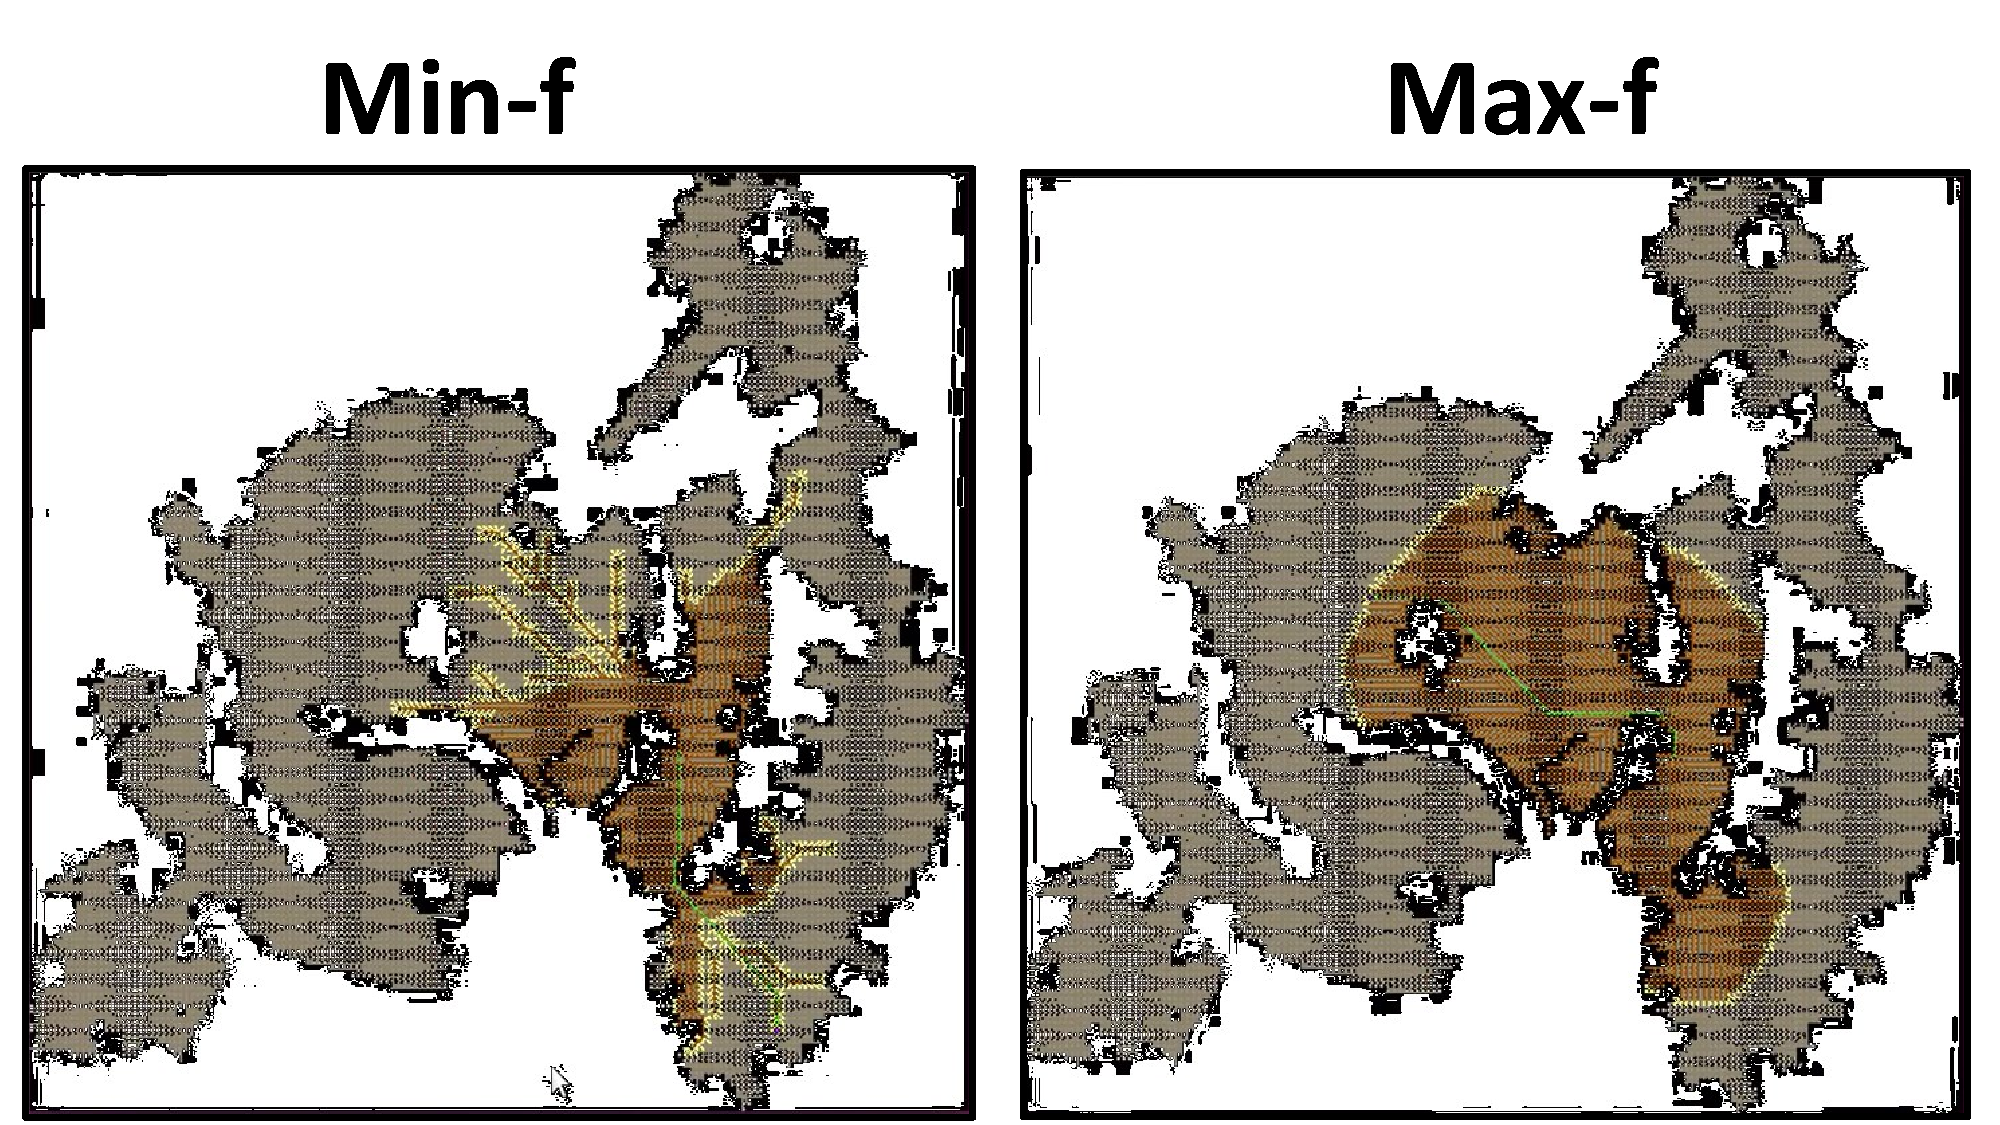
\includegraphics[width=\columnwidth]{min-vs-max}
    \caption{An example of running \kastarmin{} (left) and with \kastarmax{} (right). The yellow parts represent the states in \open{}, the brown parts represent the states in \closed{}.
    To see a running example of how \open{} changes throughout the search in  this example see the vidoes in the following URLs \url{http://tinyurl.com/ze29tb4} (for \kastarmax) and
    \url{http://tinyurl.com/zawrmtd} (for \kastarmin).
}
    \label{fig:min-vs-max}
\end{figure}


An interesting observation is that \kastarmax{} is faster than Eager
\kastarmin{} when the number of goals is large (see $k=64$ and $128$). To
explain this, consider the illustrations in Figure~\ref{fig:min-vs-max}. They
show an example of running \kastarmin{} (left) and \kastarmax{} (right) on the
same \kgs{} instance. The yellow points represent states in \open{}, the brown
points represent states in \closed{}, the graph points are states that were not
generated so far, and the white points and the black points are impassable
obstacles. As can be seen, the behavior of \kastarmin{} and \kastarmax{} are
different: \kastarmin{} runs greedily towards prospective goals, showing clear
trajectories protruding from the search frontier, while \kastarmax{}
demonstrates a behavior that is more similar to uniform cost search. This
occurs  because when a child is generated in \kastarmin{}, if it is closer to
the closest goal than its parent then it will be expanded next, resulting in
these protruding DFS-like trajectories towards the goal. By contrast, in
\kastarmax{} even if a state generates a child state that is closer to the
closest goal, it still may not be expanded because it is further from some
other goal. This results in having \kastarmax{} behaving in a somewhat similar
manner to UCS, and thus for large number of goals its \open{} will contain
fewer states than \kastarmin{}.\footnote{Having fewer 
states in \open{} also impacts the costs $C_{gen}$ and $C_{r}$, since we implemented
\open{} using a binary heap, and thus the runtime of reordering \open{} and
inserting states into \open{} depends on the size of \open{}. Indeed, the
assumption that $C_{gen}$ and $C_r$ are constant throughout the search is only
an abstraction of the true costs, which depends on the exact implementation.}





%\roni{Probably there's a nicer way to explain this.} [[AF: Yes there is. We need to think]] This behavior results in \kastarmin{} having a weaker duplicate detection phase compared to \kastarmax{}, resulting in a bigger \open{} and thus more generated states. \roni{Can anyone explain why Lazy \kastar{} generates more states?} [[AF: Lazy should be identical to \kastarmin{}. Maybe they had different tie breaking?]]


%\begin{figure}
%   \includegraphics[width=0.45\columnwidth]{Capture-minf.PNG}
%   \includegraphics[width=0.45\columnwidth]{Capture-maxf.PNG}
%   \caption{XXx}
%   \label{fig:min-vs-max}
%\end{figure}


\subsubsection{The Impact of the Distance between Goals}

\begin{figure}
    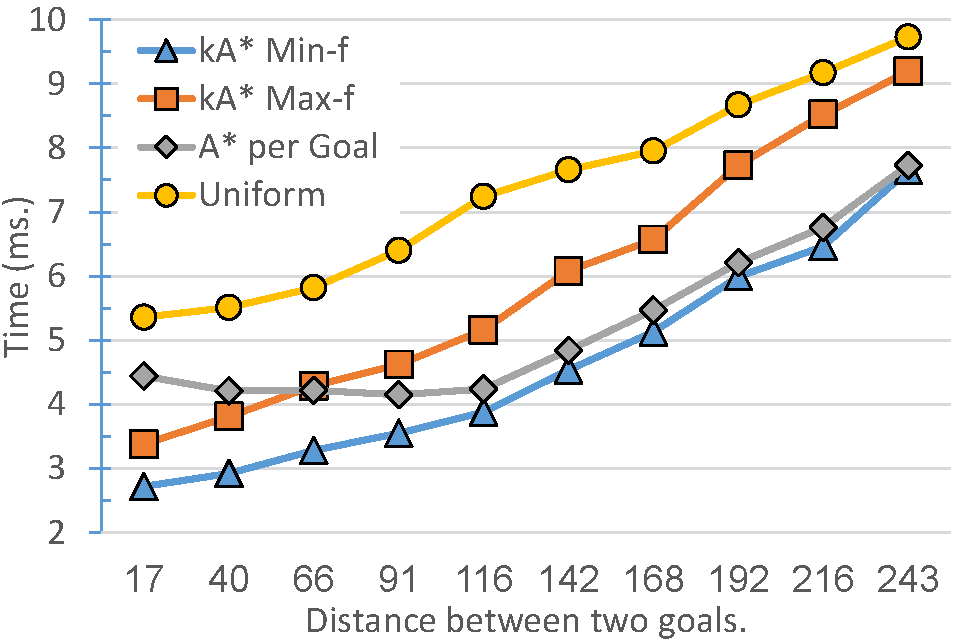
\includegraphics[width=\columnwidth]{G0-G1_cropped.pdf}
    \caption{This figure plots the runtime (in ms.) of the different \kgs{} algorithms as a function of the distance between the goals, for a \kgs{} problem with two goals ($k=2$).}
    \label{fig:2-goal}
\end{figure}



In the second type of experiments we performed, we focused on \kgs{} problems
with two goals ($k=2$), and investigated the impact of the distance between
these goals on the effectiveness of the evaluated algorithms.

%\roni{TODO: Fill in with Meir: how was the random walks performed, how was the binning, etc.}


The results are given in Figure~\ref{fig:2-goal}. The $x$-axis is the distance
between the goals, and the $y$-axis shows the average runtime in milliseconds
of the different algorithms. We compared Lazy \kastarmin{}, \kastarmax{},
\kxastar{}, and UCS. We observe several trends. First, for a 2 goal problem it
is clear that uniform cost search is the worst option. This is reasonable as
UCS is only effective when the number of goals is large (since it does not use
a heuristic).
%This is reasonable, as it does not use a heuristic to guide its search and the number of goals is small.
Second, observe that when the goals are close to each other, both \kastarmin{}
and \kastarmax{} outperform \kxastar{}. This matches our analysis
(Section~\ref{sec:theoretical-analysis}), where if the goals are close to each
other we expect that many states will be expanded by both independent \astar{}
searches, which is  exactly the redundancy \kastar{} was designed to solve.
More formally, when the goals are close to each other, then the intersection of
$Gen(\text{\astari{1}})$ and $Gen(\text{\astari{2}})$ will be large and so
$|Gen(\text{\astari{1}})\cup Gen(\text{\astari{2}})|$ will be significantly
smaller than $|Gen(\text{\astari{1}})|+|Gen(\text{\astari{2}})|$, providing an
advantage to \kastarmin{} (see Table~\ref{tab:time-analysis}). Following this
explanation, we observe that as the goals chosen become distant from each other
(going right on the $x$ axis of Figure~\ref{fig:2-goal}), we see that the
advantage of \kastar{} over 2 \astar{} searches diminishes. Indeed, the
performance of \kastarmin{}  and \kxastar{} converge when the goals are
furthest from each other. Lastly, we observe that \kastarmin{} dominates
\kastarmax{} and in general all other approaches, always being better or on par
with the other algorithms.

\subsubsection{The Impact of Using Stronger Heuristics}

\begin{figure*}
    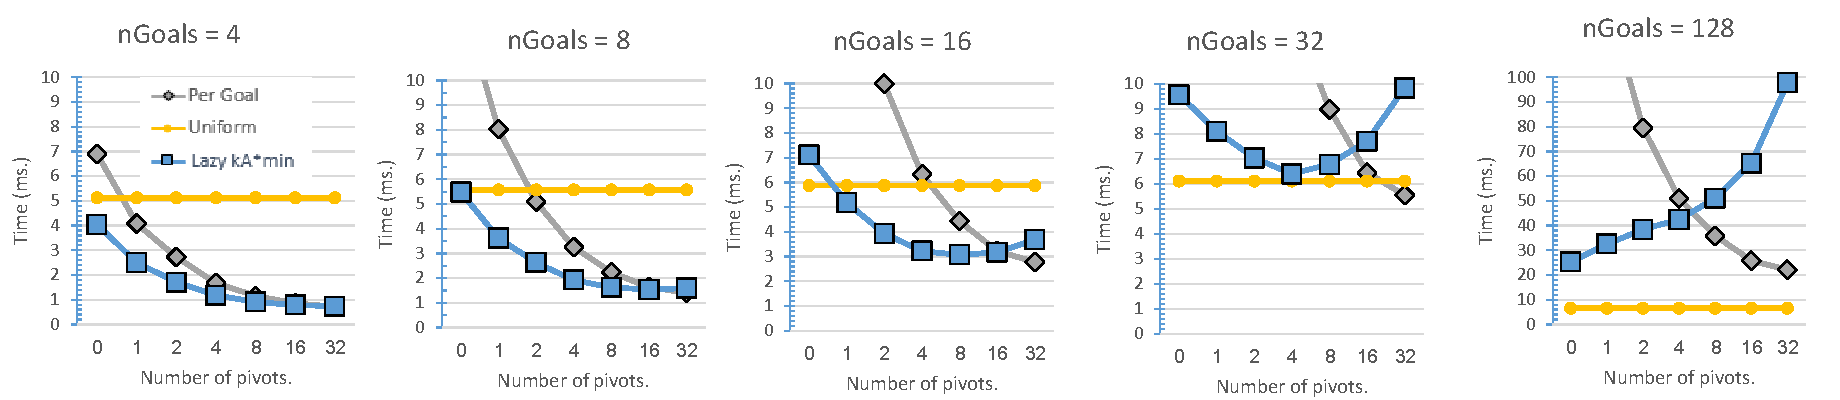
\includegraphics[width=\textwidth]{heuristic-power_cropped.pdf}
\caption{The runtime of Lazy \kastarmin{}, \kxastar{}, and UCS for different
number of goals (the different plots) and difference number of pivots using in
the heuristic computation. With more pivots, the heuristic is more accurate but
slower to compute.}
    \label{fig:dh-results}
\end{figure*}


Next, we evaluated the impact of using a stronger, more accurate heuristic, on
the performance of the proposed \kgs{} algorithms. To this end, we used
differential heuristics
(DH)~\cite{goldberg2005computing,ng2002predicting,sturtevant2009memory} instead
of Octile distance. DH is a more sophisticated memory-based heuristic for grid
pathfinding that works as follows. A set of states (cells in the grid) are
chosen  referred to as the {\em pivots}. Then, in a pre-processing step, we
compute and store in memory the shortest path between every state and these
pivot states. When computing the heuristic for a state that is not part of
these states, one can use the triangle inequality to obtain an admissible
heuristic. For more details,
see~\cite{goldberg2005computing,ng2002predicting,sturtevant2009memory}.
Importantly, adding more pivots results in a more accurate heuristic, but one
that takes longer time to compute.


Thus, DH is especially useful for our analysis, as it can be tuned to more
accurate and more costly to compute. The results of Lazy \kastarmin{},
\kxastar{} and UCS are given in Figure~\ref{fig:dh-results}. The different
plots show the results for 4, 8, 16, 32, 64, and 128 goals.The $y$ axis shows
the average runtime in milliseconds and the $x$ axis shows the number of pivots
used for computing the heuristic. As expected, the runtime of UCS is unaffected
by the number of pivots, since it does not use a heuristic. Also, if we fix the
number of pivots and observe the impact of increasing the number of goals, the
benefit of using heuristic search over plain UCS diminishes. Eventually, when
solving for 128 goals, UCS dominates both \kastarmin{} and \kxastar{}. This
follows the same trends observed for the Octile distance results given in
Table~\ref{tab:pathfinding-runtime}, and the explanation we provided for these
results hold here too.
%is the same as tehre. %solving for large number of goals eventually

%[[AF: in the figure please reword the "per Goal" to be consistent with the terminology in this paper. In other places too.]]

Next, consider the impact of adding pivots -- i.e., using a stronger but more
costly heuristic. For \kxastar{}, we observe that adding pivots always helps
reducing runtime. For \kastarmin{}, however, adding pivots improves runtime
only for cases when the number of goals was not very large. For example, when
$k=32$, using more than 4 pivots actually degrades the performance of
\kastarmin{}. These results conform with out theoretical analysis: adding
pivots increases $C_h$, which is incurred more times in \kastarmin{} than in
\kxastar{} (see Table~\ref{tab:time-analysis}).

%This is done  \kastar{} and \kxastar{} in


\subsection{Pancake Puzzle}




Next, we present the results for the pancake puzzle. The heuristic used was the
GAP heuristic~\cite{helmert2010landmark}, adjusted so that it is suitable for
different goal states.
%\roni{Meir: what was the heuristic used? how were the states generated? how many instances?}
We experimented with 1, 2, 4, 8 and 16 goals ($k$). For every $k$ we generated
100 random instances, where goal $g_1$ was the standard pancake goal state
(where the pancakes are stacked by size) and the other goals are random
permutations. %[[AF: so in fact, it is equivalent to the case where they are all random permutations]]\roni{Not sure why we should mention this?}


\begin{table}[]
    \centering
    \begin{tabular}{|r|r|r|r|r|}
        \hline
        \multicolumn{1}{|l|}{}            & \multicolumn{2}{c|}{Runtime (ms.)}                                       & \multicolumn{2}{c|}{Generated} \\ \hline
        \multicolumn{1}{|c|}{\# Pancakes} & \multicolumn{1}{c}{\kastarmax{}} & \multicolumn{1}{c|}{Uniform} & \multicolumn{1}{c}{\kastarmax{}} & \multicolumn{1}{c|}{Uniform} \\ \hline
        6                               & 0.34                                      & 0.46                        & 994                                       & 2,287                       \\
        7                               & 2.57                                      & 4.06                        & 8,617                                     & 21,059                      \\
        8                               & 22.95                                     & 40.25                       & 74,745                                    & 188,946                     \\
        9                               & 410.81                                    & 717.64                      & 787,481                                   &
        1,973,420\\
        \hline
    \end{tabular}
    \caption{Running time (in ms.) and number of generated states for solving \kgs{} with two goals
        in the Pancake puzzle domain using UCS and \kastarmax{}.}
    \label{tab:pancake-max-uniform}
\end{table}


The first result we report is that UCS and \kastarmax{} could not solve even
small-sized problems even for $k=2$. Average runtime and number of states
generated  for $k=2$ and pancakes of size up to 9 are given in
Table~\ref{tab:pancake-max-uniform}. These results are not surprising, because
in exponential domains running a search without a heuristic is not practical,
and \kastarmax{} can behave similar to UCS (as shown also in
Figure~\ref{fig:min-vs-max}).


\subsubsection{The Impact of Varying the Number of Goals}


\begin{table*}[]


            \centering
        \begin{tabular}{|r|r|r|r|r|r|r|r|r|}
            \hline
            & \multicolumn{4}{c|}{{\bf 10 Pancakes}} & \multicolumn{4}{c|}{{\bf 20 Pancakes}}    \\
            \hline
            & \multicolumn{2}{c|}{Runtime (ms.)}   & \multicolumn{2}{c|}{Generated}    & \multicolumn{2}{c|}{Runtime (ms.)}   & \multicolumn{2}{c|}{Generated}    \\
            \hline
            $k$ & \kastarmin{} & \kxastar{} & \kastarmin{} & \kxastar{} & \kastarmin{} & \kxastar{} & \kastarmin{} & \kxastar{}  \\ \hline

1           & 0.09                  & \textbf{0.08}       & \textbf{190}          & \textbf{190}        & 4.24                  & \textbf{4.17}       & \textbf{7,324}        & \textbf{7,324}      \\
2           & 0.20                  & \textbf{0.16}       & \textbf{363}          & 368                 & 9.75                  & \textbf{7.81}       & \textbf{13,794}       & 13,828              \\
4           & 0.51                  & \textbf{0.35}       & \textbf{755}          & 788                 & 21.74                 & \textbf{13.73}      & 25,154                & \textbf{24,982}     \\
8           & 1.18                  & \textbf{0.67}       & \textbf{1,364}        & 1,512               & 66.63                 & \textbf{30.14}      & \textbf{53,268}       & 53,790              \\
16          & 3.24                  & \textbf{1.35}       & \textbf{2,645}        & 3,058               & 206.03                & \textbf{59.51}      & \textbf{103,674}       & 105,863     \\ \hline
    \end{tabular}
    \caption{The average runtime and average number of states generated in the pancake experiments, for \kastar{} with \minf{} and for running $k$ independent \astar{} searches. Best results per $k$ are highlighted in bold.}
    \label{tab:pancake-minf-k-searches}
  \end{table*}



\kastarmin{} and \kxastar{} were able to solve larger pancake puzzle instances.
Therefore, we were able to evaluate  the impact of varying the number of goals
on their performance. Table~\ref{tab:pancake-minf-k-searches} presents their
results for the 10 and 20 pancakes puzzle and different number of goals. As
expected, \kastarmin{} usually generates fewer states. Nonetheless, the
difference, in terms of number of states generated, is very small in this
domain.  Moreover, the runtime of \kastar{} is constantly larger than the
runtime of \kxastar{}, and the difference between them grows when the number of
goals increase. This is because in exponential domains the intersection between
the sets of states generated by each search is small compared to size of the
last $f$ layer of each search which is quite large. 

%\roni{Meir and Ariel, I'm looking for a nicer explanation. Any thoughts?}\roni{I am not sure how the ``denied'' column help explain this. If we have many denied states doesn't it mean that the intersection was actually large? }[[AF: I added some text but I think it is OK]]


\begin{figure}
    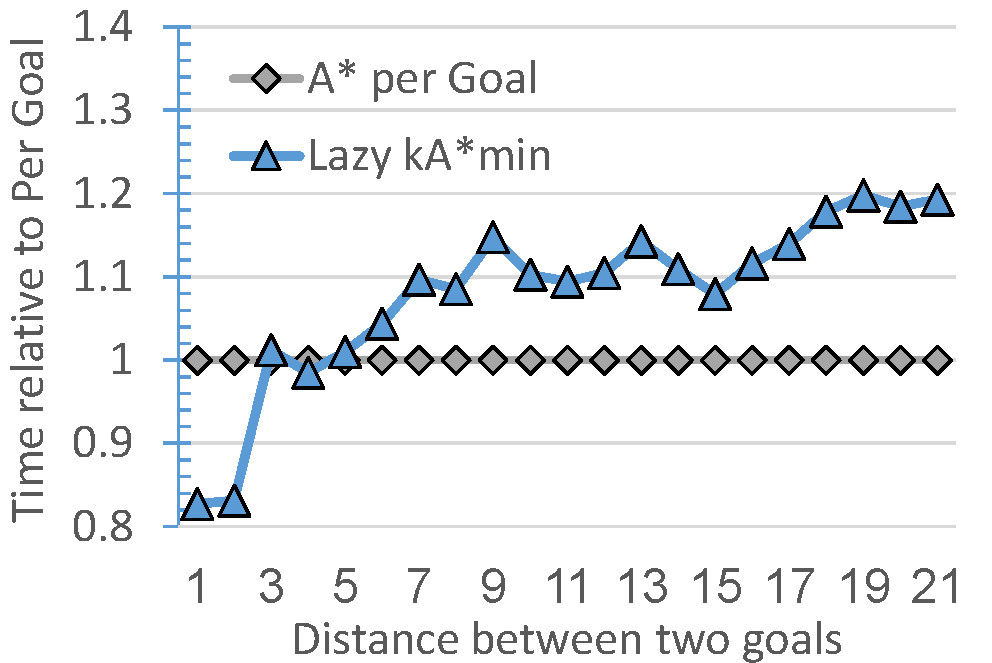
\includegraphics[width=\columnwidth]{pancake-goal-distance_cropped.pdf}
    \caption{10 pancake domain. Runtime as a function of the distance between the goals in \kgs{} with two goals.}
    \label{fig:2-goal-pancake}
\end{figure}

\subsubsection{The Impact of the Distance between Goals}

Next, we evaluated the impact of varying the distance between the goals,
focusing on \kgs{} problems with two goals. To do so, we generate 1,000 problem
instances for this experiment by choosing the standard goal state (where all
pancakes are ordered nicely) and performing a limited number of random walks
from it: 10 problem instances were generated by a single random step from the
standard goal, the subsequent 10 problem instances were generated by two random
steps from the standard goal, and so on. Then, each instance was solved
optimally to find the exact distance between the goals, and the results of
instances with similar distance were bucketed together.



%To gain a deeper insight into the behavior of the various \kgs{} algorithm in this domain, we performed additional experiments.

Figure~\ref{fig:2-goal-pancake} plots the runtime of Lazy \kastarmin{} and
\kxastar{} for these \kgs{} instances with different distances between them
(depicted in the $x$-axis). Here, we show the relative runtime of \kastarmin{}
compared to \kxastar{}. So values smaller than one correspond to cases where
\kastarmin{} was faster than \kxastar{} and values larger than one correspond
to cases where \kxastar{} was faster.

As we observed in the grid path finding domain, when the goals are very close,
\kastarmin{} is better that \kxastar{}, as there is a large intersection
between the states generated by the individual \astar{} searches. However, we
observe here that unlike the grid path finding domain, the advantage of
\kastarmin{} quickly disappears, and for cases where the goals are more than 5
steps apart it is better to use \kxastar{}. To explain this, note that the
pancake puzzle is an exponential domain. Therefore, even if the two goals are
relatively close to each other, the search spaces corresponding to finding each
of them can be them may have a relatively small overlap. Consequently,
\kastarmin{} will perform poorly compared to \kxastar{}.

% This supports our analysis, as in exponential domains a small distance between the goals can result in needing a very large number of unique states to expand per goal.



To conclude our experimental results, we observed the following trends:
\begin{enumerate}
    \item Eager \kastarmin{} usually outperforms \kastarmax{}, but not always. Lazy \kastarmin{} outperforms both.
    \item When the number of goals becomes very large, simply running UCS is the best option, as it does not spend time on heuristic computations.
    \item In the grid pathfinding domain, which is a polynomial domain, many states are generated by more than one search, and consequently \kastar{} is advantageous compared to \kxastar{} searches.
    \item In the pancake domain, which is an exponential domain,
    only relatively few states were generated by more than one search,
    and so running $k$ individual searches (\kxastar{}) is usually faster than running
    \kastar{}, unless the goals are very close to each other.
\end{enumerate}




\section{Related work}
\label{sec:related-work}

\kgs{} is similar to many previously studied problems. As mentioned in the
introduction, \kgs{} is different from TSP in that in TSP the task is to find a
shortest path that passes through a set of vertices, while in \kgs{} that task
is to find $k$ shortest path, one to each vertex.
%In that sense it is similar to the minimal spanning tree (MST) problem, but we only require optimal path to a selected set of $k$ vertices and not to all vertices (as in MST).


\kgs{} is also different from a disjunction of $k$ goals, i.e., from the case
where there are $k$ possible goals and the task is to find the lowest cost path
to the closest one. Unlike this case of a disjunction of $k$ goals, in \kgs\ we
must find the shortest path to each of the goals, and not just to the closest
one.


Somewhat related is the work on {\em multi-objective search}, where we have
multiple objectives function that we wish to optimize. For example, in a
navigation application one may want to optimize for path length and also for
ease of navigation. An optimal solution to a multi-objective optimization
problem is usually a solution that is Pareto-optimal, and it is often the case
that one would like the set of all Pareto-optimal solutions. This is
fundamentally different from \kgs{}, where we have a single optimization
criteria -- we must have the lowest-cost path to all $k$ goals.

The \kgs{} problem is related to the problem addressed by incremental search
algorithms such as Lifelong Planning \astar{}~\cite{koenig2004lifelong},
D*-Lite~\cite{koenig2005fast}, and Path-Adaptive
A*~\cite{hernandez2015reusing}. Incremental search algorithm are designed to
solve a sequence of search problems, where the start and goal of these search
problems are the same, but the underlying graph has changed. The key idea in
incremental search algorithms is to re-use information from previous searches
to solve faster the current search problem. However, unlike the incremental
search setting is different from \kgs{}: in incremental search we have one goal
and the environment is dynamic, while in \kgs{} we have $k$ goals but assume
the environment does not change.

Another related problem is the moving-target search
problem~\cite{koenig2007speeding,ishida1991moving}. Moving-target search
problems are search problems where the goal changes during the search. This is
different from \kgs{} where the goals do not change during the search, but we
know upfront the $k$ goals. In the next section we discuss possible directions
for future research in which \kgs{} is compiled to a moving target
search problem or an incremental search setting. %existing incremental search algorithms and existing moving-target search algorithms are adap


\section{Conclusion and Future Work}

In this work we studied the \kgs{} problem, and analyzed two fundamental
approaches for solving it: $k$ single-goal searches and a single search for $k$
goals. We analyzed the deficiencies of $k$ single-goal searches and formalized
\kastar{}, a single algorithm that searches for $k$ goals together. Several
variants of \kastar{} were presented: \kastarmax{}, Eager \kastarmin{},
Eager$^+$ \kastarmin{}, and Lazy \kastarmin{}. Given an admissible heuristic,
both Eager and Lazy \kastarmin{} are sound and complete, and if the heuristic
is consistent so is \kastarmax{}. We then analyzed all the proposed algorithms
theoretically, comparing their memory requirements and runtime. Finally, we
performed an experimental study on two representative domains: one with a state
space that is polynomially in the input and one with a state space that is
exponential in the input. Empirically, we showed that Lazy \kastarmin{}
dominates the other \kastar{} variants. In addition, our results suggest that
in polynomial domains it is usually the case that running \kastar{} is better
than \kxastar{}, but in exponential domains \kxastar{} is usually better.
Finally, if the number of goals is very large then running UCS is the best
option.



This work is, to the best of our knowledge, the first study of using heuristic
search techniques to solve \kgs{}. There are several exciting directions for
future work. First, we only explored in this work how to avoid some of the
redundant computations done when performing $k$ individual searches. As
mentioned briefly in Section~\ref{sec:k-one-goal}, a different way to benefit
from searching for multiple goals is that while searching for one goal one can
learn valuable information about the underlying graph, which may later be used
to improve the search. This can include, for example, using learning techniques
to improve the quality of the heuristic.

We give two possible directions for future work where such learning from
experience can occur. One way to do so is to improve the available heuristics
by using knowledge about the shortest path found so far. For example, in
undirected graphs the difference between the heuristic for one goal and the
heuristic between the goals is actually an admissible heuristic that may be
more accurate than the given heuristic $(h_1,\ldots h_k)$. 
%[[AF: better explain what you mean. What is your new heuristic? Define it precisely.]]\roni{No, this is a future work section, not the body of the paper. Defining things precisely would be too formal for this part of the paper.}
This idea is
inspired from memory-based heuristics used by path finding
algorithms~\cite{sturtevant2007memory,sturtevant2009memory,goldenberg2011theCompressed}.


Another way to learn information about the search space is to compile \kgs{} to
an incremental search problem. This can be done by adding an artificial vertex
that is connected to all goals, and running the search from this goal to the
start state. Then, every iteration of the incremental search algorithm will
change the weight of the edges from the artificial goal to the actual goal,
setting the edge to exactly one goal with zero weight and all other edges as
unpassable. This compilation may enable using incremental search algorithm such
as Path-Adaptive A*~\cite{hernandez2015reusing} to solve the \kgs{} problem. A
challenge in such an approach is how to choose the order of goals that will be
solved, so as to optimize the amount of information learned between searches.
Also, we believe that a similar approach for solving \kgs{} can be done by
compiling it to a moving target search problem.





% \begin{figure}[!htbp]
%   \centering
%   \includegraphics[width=1\hsize]{filename.eps}
%   \caption{caption} \label{fig:label}
% \end{figure}

\section*{Acknowledgements}

Financial support for this research was in part provided by Israel Science
Foundation (ISF) grant \#417/13.

\bibliographystyle{abbrv}
\bibliography{library}

\end{document}
